\documentclass{sintefbeamer}

% packages, font, color, and newcommands
\usepackage{amsfonts, amsmath, oldgerm, lmodern, bm}
% \usepackage[font={footnotesize}]{caption}
\usepackage{natbib}
\usepackage{url}
\usepackage{tikz}
\usepackage{amssymb}
\usepackage{amsmath}
\usepackage{amsthm}
\usepackage{mathrsfs}
\usepackage{empheq}
\usepackage{mdframed}
\usepackage{bm}
\usepackage{animate}
\usepackage{xcolor,colortbl}
\usepackage{graphicx}
\usepackage{stmaryrd}
\usepackage{amsmath}
\usepackage{animate}
\usepackage{array}
\usepackage{cancel}

\tikzset{  node distance=3cm and 5cm,
every node/.style={align=center, font=\sffamily},
box/.style={ rounded corners, minimum width=3.5cm, minimum height=1cm, text centered,fill=sintefblue!15},
arrow/.style={-{Latex}, thick}}
\bibliographystyle{apalike}

\useoutertheme{miniframes}
\usefonttheme{serif}

\usetikzlibrary{arrows.meta,
                chains,
                calc,
                positioning,
                shapes.geometric,
                backgrounds}

\title{Statistical modeling of disperse two-phase flows : application to buoyancy -driven droplets suspensions}
\subtitle{Doctoral seminar}

\author
{\href{http://basilisk.fr/sandbox/fintzin/Rising-Suspenion/RS.c}
{\underline{N. Fintzi}\footnote{IFP \'Energies Nouvelles, France}$^{,2}$}, 
JL. Pierson$^1$ and 
S. Popinet\footnote{Sorbonne Universit\'e, France}
}


\titlebackground{image/800good.png}

% document body
\addtobeamertemplate{navigation symbols}{}{%
    \usebeamerfont{footline}%
    \usebeamercolor[fg]{footline}%

    \insertframenumber/\inserttotalframenumber
}


% \includeonlyframes{current}


\begin{document}

{\setbeamertemplate{headline}{}
% \setbeamertemplate{footline}{}
\setlength{\headheight}{0pt}
\maketitle
}

\section{Context}


\begin{frame}
  \frametitle{Why studying emulsions ? }
  \centering
  {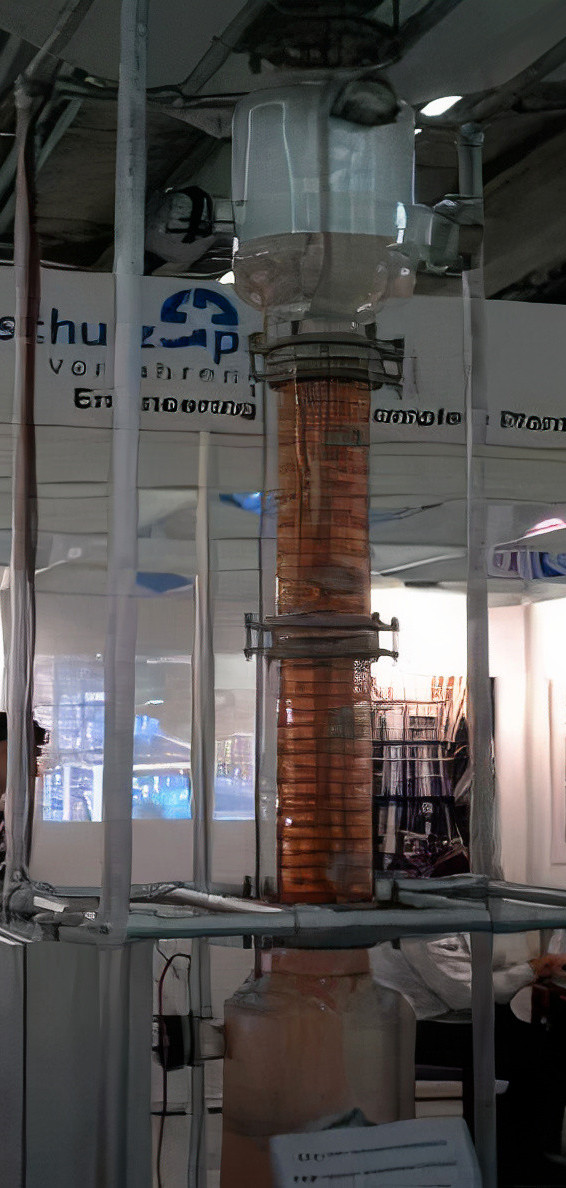
\includegraphics[height=0.3\textwidth]{image/liq-liq_LE_auto_x5.jpg}}
  \uncover<2->{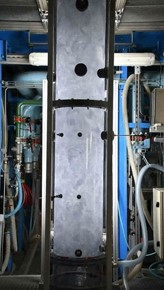
\includegraphics[height=0.3\textwidth]{image/Image2.jpg}}
  \uncover<3->{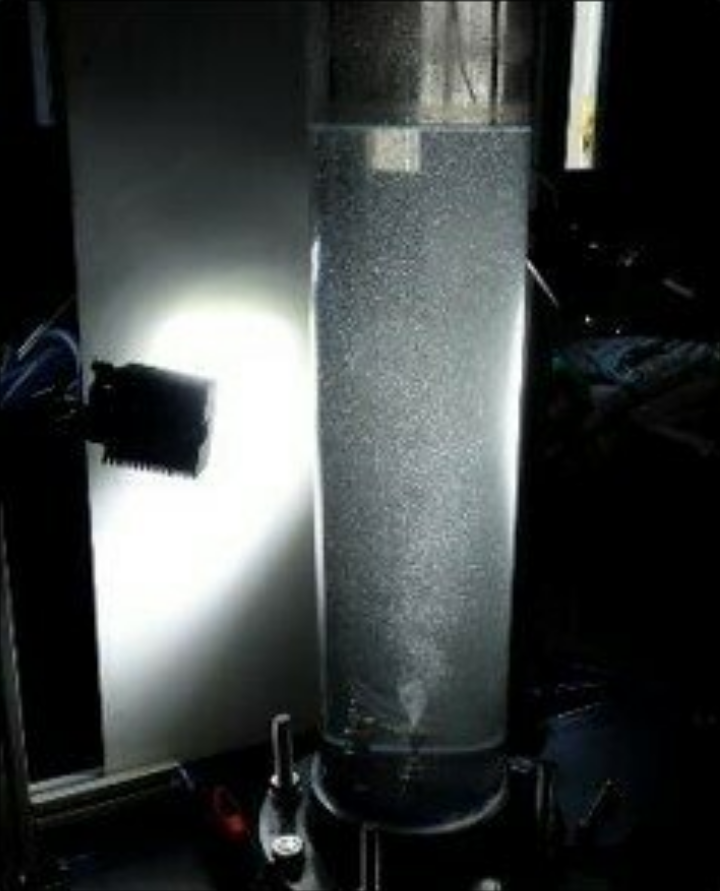
\includegraphics[height=0.3\textwidth]{image/flo.png}}
  % \uncover<4->{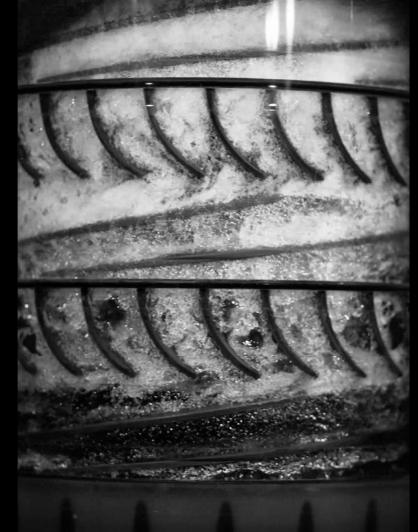
\includegraphics[height=0.3\textwidth]{image/Image4.png}}
  \begin{itemize}
    \item<1-> Liquid-liquid separation processes
    \item<2-> Bubbles columns
    \item<3-> Flotation columns 
    % \item<4-> Multiphase pumps
    \item<4-> And other\ldots
  \end{itemize}
\end{frame}


\begin{frame}
  \frametitle{Needs ?}
  
  \centering
  \textbf{\underline{Predict global hydrodynamics}}

  \uncover<2->{
  \begin{itemize}
    % \item Predict global hydrodynamics% in dispersed bubbly flows and emulsions: % (interphase forces etc\ldots).
    % \begin{itemize}
      \item Velocity of each droplet ? 
      % \item volume fraction ?  
      \item Size of the droplets ?  
      \item Deformations of each droplet ?  
      \item \ldots
    % \end{itemize}
  \end{itemize}
  }


\end{frame}

\begin{frame}
  \frametitle{Problem ! \uncover<3->{Upscaling ?} }
      \centering
      \setbeamercovered{transparent=10}

      \begin{tikzpicture}
        \node (img) at (0,0) {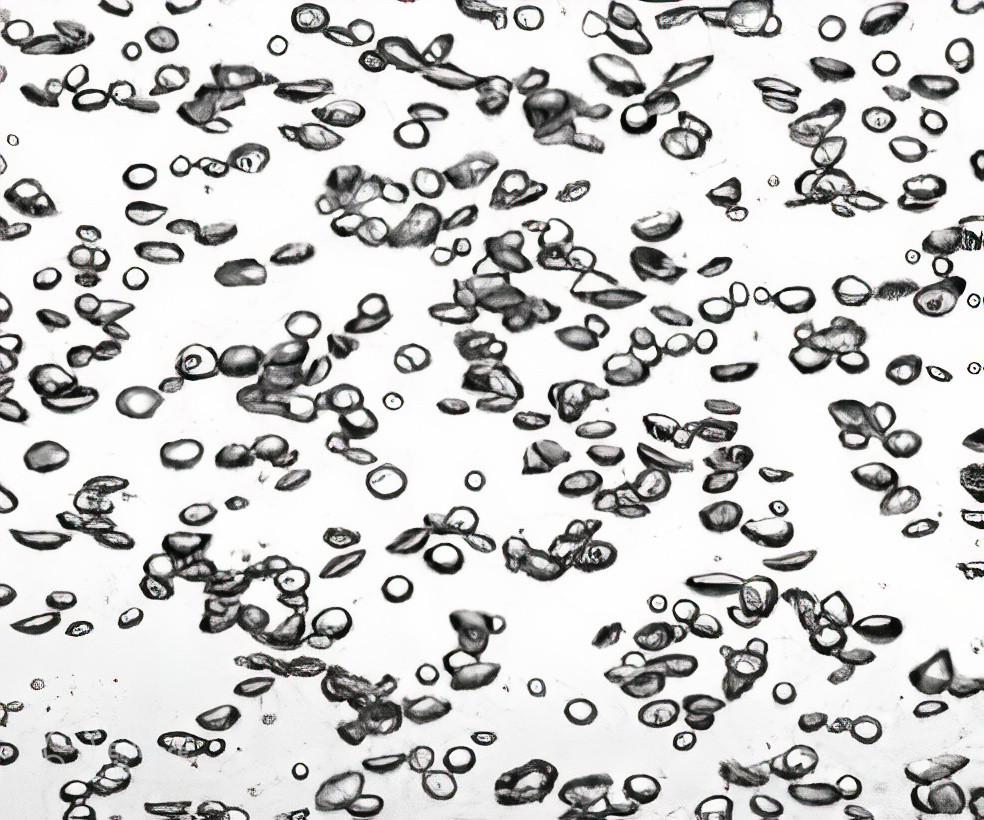
\includegraphics[height=0.25\textwidth]{image/bubbles_4x.jpg}};
        \node[above] (title1) at (0,0.125\textwidth) {\textbf{Local description} \citep{Dung_Waasdorp_Sun_Lohse_Huisman_2023}};
        \uncover<3->{
        \node[text width=6cm] (itm) at (0.55\textwidth,0) {
          \begin{itemize}
            \item Volume fraction of droplets ?  
            \item Mean velocity of each phase ? 
            \item \ldots
          \end{itemize}
          };
          \node[above] (title2) at (0.55\textwidth,0.125\textwidth) {\textbf{Macroscopic description}};
        \draw[arrow,very thick] (img) -- (itm)node[midway,above]{Upscaling};
        }
        \uncover<1->{
          \node[yshift=-3em,box,text width=5cm] (eq1) at (0,-0.125\textwidth) {Navier-Stokes equations and Newton second-law};
          \draw[arrow](img) -- (eq1);
        }
        \uncover<4>{
          \node[yshift=-3em,box] (eq2) at (0.55\textwidth,-0.125\textwidth) {\underline{Average} Navier-Stokes equations};
          \draw[arrow](itm) -- (eq2);
        }
      \end{tikzpicture}

      \vfill

      \uncover<2->{
      $\to$\textbf{Problem !} For large number of droplets these predictions are impossible !
      }
\end{frame}


\begin{frame}
  {Mathematical modeling of dispersed two-phase flows }
    
  
  \begin{tikzpicture}
  
  
  \node[box] at (0,3)(lagrangian) {Lagrangian description of droplets \\ $\sum \textbf{F} = \ddt (m_i\textbf{u}_i)$};
  \node[box] at (8,3)(Eulerian) {Eulerian description of the continuous phase \\ $\div\textbf{u}= 0$\\ $\rho (\pddt + \textbf{u}\cdot\grad)\textbf{u} = \div\bm\sigma + \rho\textbf{g} $};
  \uncover<2->{
  \node[box] at (0,0)(kinetic) {``Kinetic Theory''-like models \\ (Simonin 1996)};
  \node[box] at (8,0)(twofluid) {Two-Fluid formulation \\ (Drew 1983)};
  \draw[arrow] (lagrangian) -- (kinetic) node[midway, right] {Statistical averaging};
  \draw[arrow] (Eulerian) -- (twofluid) node[midway, right] {Statistical  averaging};
  }
  \uncover<3>{
  \node[box] at (4,-2.7)(unify)  {Hybrid Multiphase Flow model (Lhuillier 1992, Zhang et Prosperetti 1994)};
  \draw[arrow] (twofluid) -- (unify);
  \draw[arrow] (kinetic) -- (unify);
  \draw[arrow] (twofluid) -- (unify);
  \node[below =0.5cm of kinetic, text width=4.5cm] (desc1) {\textit{Describes the mean particle trajectories}};
  \node[below =0.5cm of twofluid, text width=4.5cm] (desc2) {\textit{Models the average continous phases behaviour}};
  }
  \end{tikzpicture}
  
  \end{frame}

\begin{frame}
\frametitle{Averaged hybrid model }

  \begin{itemize}
    \item Provide: \uncover<1->{
      \begin{itemize}
        \item Averaged velocity fields 
        \item Volume fraction field 
        \item Averaged pressure field 
        \item \ldots
      \end{itemize}
      }
    \item Require: \uncover<2>{ \underline{Sub-scale models}
    \begin{itemize}
      \item Forces between dispersed and continuous phases ? 
      \item Frequency of droplets coalescence and breakup:
      \begin{itemize}
        \item Describe the interactions between pairs of droplets
        \item Predict the interaction frequency
        \item Predict the film drainage time
        \item etc...
      \end{itemize}
      \item Local velocity fluctuations
    \end{itemize}}

  \end{itemize}

\end{frame}




\begin{frame}
  \centering
  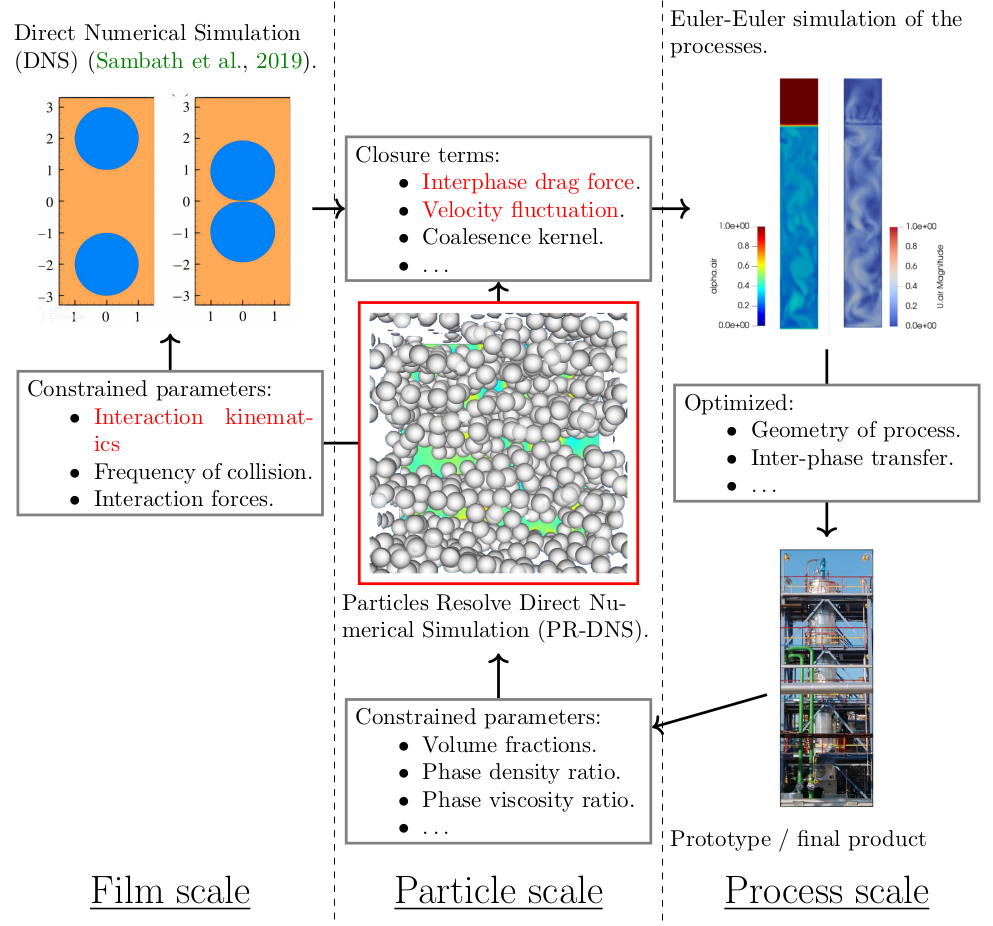
\includegraphics[height=1.1\textheight]{image/start.png}
\end{frame}



\begin{frame}
  {In this work we focus on three aspects of the problem :}
  \Large
  \setbeamercovered{transparent=15}
  \begin{enumerate}
    \item<1-3> Mathematical modeling of \textbf{dispersed two-phase flows} using ``kinetic-theory''-like approach. 
    \only<2>{ 
      \begin{itemize}
        \item Solid particles suspensions: \citet{jackson1997locally,zhang1994ensemble}\ldots
        \item Fluid inclusions: \citet{lhuillier1992ensemble,morel2015mathematical}
        % \item How to model non-spherical and deforming particles?
        % \item How to model surface properties of droplets ? 
        \item Identification of the closure terms of the ``Hybrid-model''. 
      \end{itemize}
      }
      \item<4-6,8> \underline{Theoretical} and \underline{Numerical} investigations of buoyant emulsions to provides subscale-model for step (\textcolor{sintefblue}{1.}). 
      \only<5>{
        \begin{itemize}
          \item Interphase drag force model.  
          \item Turbulence models. 
          \item \ldots
        \end{itemize}
      }
    % \begin{itemize}
    %   \item Provide closure terms for the averaged Navier Stokes equations such as the Drag force, Reynolds Stresss, Particule-fluid-Particule stress \ldots 
    % \end{itemize}
    \item<7>{We use the Nearest Particule Statistics framework to explain qualitatively and quantitatively the \textbf{average interaction behaviour} between droplet pairs within a buoyant emulsion. }
  \end{enumerate}
  \setbeamercovered{transparent=0}
  \uncover<8>{\underline{{This presentation focuses exclusively on  step \textcolor{sintefblue}{2.}}}}
\end{frame}




\begin{frame}
  \frametitle{Scope of the PhD}
  \centering
  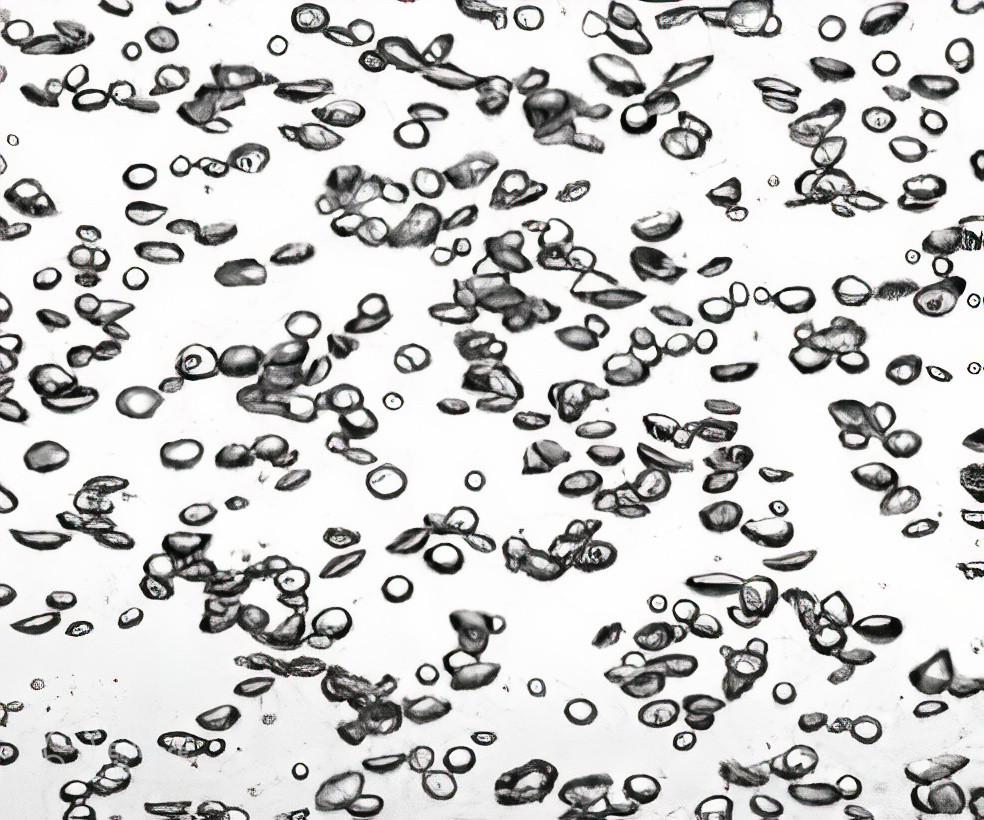
\includegraphics[height=0.3\textwidth]{image/bubbles_4x.jpg}

  \begin{enumerate}
    \item Incompressible two-phase flow with \underline{surface tension}. 
    \item We discard the chemical aspect of the problem 
    \item Mono-disperse (all droplets have same volume)
    \item Constant averaged properties.   
    % \item Quasi-steady flow  
  \end{enumerate}
  
\end{frame}


% \section{Lagrangian's description of fluid particles for kinetic-theory}
\section{Hybrid model}
\section*{}



\begin{frame}
  \frametitle{Problem statement: local scale equations}
  \underline{Mass} ($\rho_f$), and \underline{momentum} ($\rho_f \textbf{u}_f^0$) conservation in $\Omega_f$ :
\begin{align}
  \div  \textbf{u}_f^0
  &= 
  0
  \\
  \rho_f (\pddt  + \textbf{u}_f^0 \cdot \grad)
  \textbf{u}_f^0  
  &= 
  \div  \bm{\sigma}_f^0 
  + \rho_f \textbf{g}
\end{align}
\begin{itemize}
    \item The superscript $^0$ indicated that it is a local quantity.
    \item $\rho_f$  density of the continuous phase. 
    \item $\textbf{u}_f^0$ Local velocity of the continuous phase.
    \item $\bm\sigma_f^0 = -p_f^0 \textbf{I} + \mu_f (\grad \textbf{u}_f^0+^\dagger\grad \textbf{u}_f^0)$ Newtonian stress tensor of the fluid phase. 
\end{itemize}
\end{frame}

\begin{frame}
  \frametitle{Ensemble average definitions}
Ensemble average (Drew 1983): 
\href{videos/avg.mp4}{
\begin{align*}
  \phi_f [\textbf{x},t] &= \avg{\chi_f [\textbf{x},t,\FF]}\\
  \uncover<2->{\phi_f  \textbf{u}_f [\textbf{x},t] &= \avg{\chi_f \textbf{u}_f^0 [\textbf{x},t,\FF]}}\\
  \uncover<2->{\phi_f \bm\sigma_f [\textbf{x},t] &= \avg{\chi_f \bm\sigma_f^0 [\textbf{x},t,\FF]}}
\end{align*}
}
  \begin{itemize}
    \item<1-> $\chi_f$ Continuous phase indicator function ($\phi_f = 1$ in the continuous phase). 
    \item<1-> $\FF$ Random realization of the multiphase flow. 
    \item<1-> $\avg{\ldots}=\int \ldots P(\FF)d\FF$ ensemble average operator. 
    \item<1->  $\phi_f$ volume fraction of the phase $f$. 
    \item<2->  $\textbf{u}_f$ mean velocity of the continuous phase.  
  \end{itemize}
  \rule{\textwidth}{0.5pt}
  $\to$ We dropped the superscript $^0$ on $\textbf{u}^0_f[\textbf{x},t,\FF]$ to indicate that $\textbf{u}_f[\textbf{x},t]$ is a macroscopic quantity. 
\end{frame}


\begin{frame}{Averaged two-fluid model (Drew 1983)}
  Averaging the \underline{mass} and \underline{momentum} equation gives, 
  \begin{align*}
    \pddt (\phi_f \rho_f)  
    + \div (
        \phi_f \rho_f\textbf{u}_f
    )
    &= 
    0,\\
    \phi_f \rho_f (\pddt + \textbf{u}_f\cdot \grad)\textbf{u}_f
    &= 
    \underbrace{\phi_f \rho_f \textbf{g} }_\text{buoyancy}
    - \underbrace{\avg{\delta_\Gamma \bm{\sigma}_f^0 \cdot \textbf{n}}}_\text{
      \href{videos/surf_avg.mp4}{Interphase drag force}
      }
    + \underbrace{\div \bm\sigma^\text{eff}}_\text{Effective stress}
  \end{align*}
\uncover<2>{  \underline{Effective stress: } 
  \begin{equation*}
    \bm{\sigma}_f^\text{eff}
    =
    - \underbrace{\avg{\chi_f\rho_f\textbf{u}_f'\textbf{u}_f'}}_\text{Reynolds Stress}
    + \underbrace{\phi_f \bm{\sigma}_f}_\text{Mean Newtonian stress}%- n_p \textbf{M}_p
  \end{equation*}}

\begin{itemize}
  \item  $\delta_\Gamma$ Interfaces indicator function. 
  \item<2>  $\textbf{u}_f' = \textbf{u}^0_f - \textbf{u}_f$ where $\textbf{u}_f^0$ is the local (non-averaged) fluid velocity. 
\end{itemize}
\end{frame}

\begin{frame}
  {Hybrid formulation (advantage \& drawbacks)}
  \only<1>{Long story (Buyevich and Shchelchkova, 1979; Lhuillier, 1992; Zhang and Prosperetti, 1994). Basic idea :}
  \begin{equation*}
      \underbrace{\avg{\delta_\Gamma \bm{\sigma}_f^0 \cdot \textbf{n}}}_\text{
        \href{videos/surf_avg.mp4}{What is this ?}
        }
  =
  \underbrace{\pSavg[]{\bm{\sigma}_f^0 \cdot \textbf{n}}}_\text{
    \href{videos/pts_avg.mp4}{what is that ?}
    }
  - \div\pSavg[]{\textbf{r} \bm{\sigma}_f^0 \cdot \textbf{n}}
  + \frac{1}{2}\grad\grad :\pSavg[]{\textbf{rr} \bm{\sigma}_f^0 \cdot \textbf{n}}
  \ldots 
  \end{equation*}

  \only<1>{
    \begin{itemize}
      \item  $\delta_p \to \sum_i^N \delta(\textbf{x}_i - \textbf{x})$ : center of mass indicator function. 
      \item   $\avg{\delta_p} = n_p[\textbf{x},t]$ : with $n_p$ the number density. 
      \item  $S$ Surface of the droplet. 
    \end{itemize}
    }
\end{frame}

\begin{frame}
  {Hybrid formulation (advantage \& drawbacks)}
  \begin{equation*}
        \avg{\delta_\Gamma \bm{\sigma}_f^0 \cdot \textbf{n}}
    =
    \pSavg[]{\bm{\sigma}_f^0 \cdot \textbf{n}}
    - \div\pSavg[]{\textbf{r} \bm{\sigma}_f^0 \cdot \textbf{n}}
    + \frac{1}{2}\grad\grad :\pSavg[]{\textbf{rr} \bm{\sigma}_f^0 \cdot \textbf{n}}
    \ldots 
    \end{equation*}
    \vfill
    \only<1,2>{
      \textbf{Momentum}  %($m_i \textbf{u}_i = \intO[]{\rho_d \textbf{u}^0_d}$) : 
      \begin{equation*}
        \ddt(m \textbf{u})
        = 
        m \textbf{g}
        + 
        \intS[]{\bm\sigma_f^0 \cdot \textbf{n}}
      \end{equation*}}
      \only<2,3>{
      \textbf{Moment of momentum} %($\textbf{P}_i = \intO[]{\rho_d \textbf{ru}_d^0}$): 
      \begin{equation*}
        \underbrace{\ddt \textbf{P}}_\text{Shape evolution}
        % = 
        % \underbrace{\ddt}_\text{Shape evolution}
        = 
        % \underbrace{ \intO[]{ \rho_d  \textbf{w}_d^0 \textbf{w}_d^0 }
        % - \intO[]{\bm{\sigma}_d^0}
        % - \intS[]{ 
        %     \gamma (\textbf{I} - \textbf{nn})
        % }}_\text{droplets internal properties}
        \text{droplets internal properties}
        + \underbrace{\intS[]{ \textbf{r}\bm{\sigma}_f^0\cdot \textbf{n}}}_\text{External contribution}
    \end{equation*}
    %   }
    \only<3>{
      % \vspace{-4cm}
  \centering
  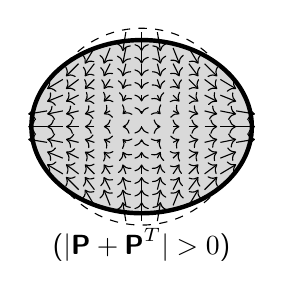
\begin{tikzpicture}[ultra thick,scale=0.5]
    \def\nRows{6}
    \def\nCols{6}
    \draw[dashed,thin] (0,0)circle(2.5);
    \draw[fill=gray!30] (0,0)ellipse(2.8 and 2.2);
    \foreach \x in {-\nRows,...,\nRows} {
        \foreach \y in {-\nCols,...,\nCols} {
            \pgfmathsetmacro\distance{veclen(\x*0.4, \y*0.4)};
            \pgfmathparse{\distance < 2.45 ? "blue" : "white"}
            \edef\colour{\pgfmathresult};
            \ifthenelse{\equal{\colour}{blue}}{                    
                \draw[thin,->](\x*0.4,\y*0.4)--++(0.08*\x,-0.08*\y);
            }
        }
    }
    \node (txt) at (0,-3){($|\textbf{P} +\textbf{P}^T| > 0$)};
\end{tikzpicture}
\hspace{1em}
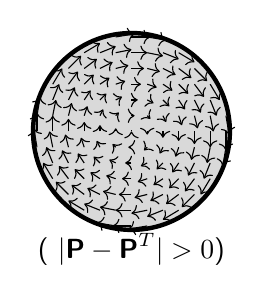
\begin{tikzpicture}[ultra thick,scale=0.5]
    \def\nRows{6}
    \def\nCols{6}
    \draw[fill=gray!30] (0,0)circle(2.5);
    \foreach \x in {-\nRows,...,\nRows} {
        \foreach \y in {-\nCols,...,\nCols} {
            \pgfmathsetmacro\distance{veclen(\x*0.4, \y*0.4)};
            \pgfmathparse{\distance < 2.5 ? "blue" : "white"}
            \edef\colour{\pgfmathresult};
            \ifthenelse{\equal{\colour}{blue}}{                    
                \draw[thin,->](\x*0.4,\y*0.4)--++(0.08*\y,-0.08*\x);
            }
        }
    }
    \node (txt) at (0,-3){( $|\textbf{P} - \textbf{P}^T|> 0$)};
\end{tikzpicture}
    }
  }
    \only<4>{
      \centering
      \begin{tabular}{|p{6cm}||p{5cm}|}\hline
        Advantages: 
        & Drawbacks: \\\hline
        \begin{enumerate}
          \item One-to-one correspondence with Lagrangian Equations
          \item Physically more understandable
          % \item Can be expressed in terms of single droplet conditional average
        \end{enumerate}
        &
        \begin{enumerate}
          \item Valid only for slightly inhomogeneous suspensions \citep{lhuillier1992volume}
        \end{enumerate}
        \\\hline
      \end{tabular}
    }
\end{frame}

\begin{frame}
  {Averaged \underline{mass} and \underline{momentum} averaged equations }
  \begin{align*}
    &\pddt (\phi_f \rho_f)  
    + \div (
        \phi_f \rho_f\textbf{u}_f
    )
    = 
    0,\\
    &
    \phi_f \rho_f (\pddt + \textbf{u}_f\cdot \grad)\textbf{u}_f
    = 
    \underbrace{\div \bm\sigma^\text{eff}}_\text{Effective stress}
    + \underbrace{\phi_f \rho_f \textbf{g} }_\text{buoyancy}
    \only<1>{- \underbrace{\pSavg{{\bm{\sigma}_f^0 \cdot \textbf{n}}}}_\text{Interphase drag force}}
    \only<2>{\textcolor{sintefcyan}{- \underbrace{\pSavg{{\bm{\sigma}_f^0 \cdot \textbf{n}}}}_\text{Interphase drag force}}}
  \end{align*}
  \underline{Effective stress: } 
  \begin{equation*}
    \bm{\sigma}_f^\text{eff}
    =
    \only<1>{- \underbrace{\avg{\chi_f\rho_f\textbf{u}_f'\textbf{u}_f'}}_\text{Reynolds Stress}}
    \only<2>{\textcolor{sintefcyan}{- \underbrace{\avg{\chi_f\rho_f\textbf{u}_f'\textbf{u}_f'}}_\text{Reynolds Stress}}}
    + \underbrace{\phi_f \bm{\sigma}_f}_\text{Mean Newtonian stress}%- n_p \textbf{M}_p
    \only<2>{\textcolor{sintefcyan}{+ \underbrace{ {\pSavg{{\textbf{r}\bm{\sigma}_f^0 \cdot \textbf{n}}}}}_\text{First moment} }}
    \only<1>{+ \underbrace{ {\pSavg{{\textbf{r}\bm{\sigma}_f^0 \cdot \textbf{n}}}}}_\text{First moment} }
    -\underbrace{\div [\ldots]}_\text{higher moments}
  \end{equation*}

\uncover<2>{
$\to$ Solved quantities: $\phi_f, \textbf{u}_f, \textbf{u}_p, \ldots$.

$\to$ We are looking for $\texttt{CLOSURE TERMS} = f(\phi_f, \textbf{u}_f, \textbf{u}_p, \ldots)$.}
\end{frame}


\section{The closure problem}
% % \section{}
\begin{frame}
  \frametitle{How to obtain the closure terms ?}

  \begin{tikzpicture}
    \node[box,text width=5cm] (A) at (0,0) {Ensemble average of the ``$N$-droplets problem''};
    \uncover<2->{
    \node[box,text width=8cm] (B) at (5,-2.5) {Solve the $N$-droplets problem with \textcolor{sintefred}{\underline{simulations}} or laboratory \underline{experiments}};
    \draw[arrow] (A) -- (B);
    }
    \uncover<3->{
    \node[box,text width=4cm] (D) at (10,0) {Closure models};
    \draw[arrow] (B) -- (D) node[midway,fill= white]{Measurements};
    }
    \uncover<4->{
    \node[box,text width=4cm] (C) at (5,2.5) {Reformulate into ``Single-droplet problem''};
    \draw[arrow] (A) -- (C)node[midway,fill= white]{Conditional average};
    }
    \uncover<5>{
      \draw[arrow] (C) -- (D) node[midway,fill= white]{Theoretical analysis};
    }
  \end{tikzpicture}

\end{frame}


\begin{frame}
  \frametitle{From the $N^{th}$ droplets problem to the single droplet problem:
  dispersed phase quantities}
  
    \begin{equation*}
      \underbrace{\pSavg{{\bm{\sigma}_f^0 \cdot \textbf{n}}}[\textbf{x},t]}_\text{$N$ droplets in a fluid}
      =
      \underbrace{
        n_p[\textbf{x},t]
        \intS[]{\bm\sigma^1 \cdot \textbf{n}}}_\text{
        \href{videos/one_particle.mp4}{One droplet problem}
        }
        \uncover<2>{
          = \underbrace{\frac{3\phi \mu_f}{2a^2} \left(\frac{3\lambda + 2}{\lambda + 1}\right)  \textbf{U}
          + \mathcal{O}(Re,\phi^2)
          }_\text{Hadamard-Rybczynski solution}
        }
    \end{equation*}
  \begin{itemize}
    \item $\bm\sigma^1[\textbf{z}|\textbf{x}]$ Mean stress at \textbf{z} conditioned on the presence of a droplet at $\textbf{x}$. 
    \item $n_p$ Number density. 
    \item $\textbf{U} = \textbf{u}_p - \textbf{u}_f$
  \end{itemize}
\end{frame}




\begin{frame}
  \frametitle{Direct Numerical Simulation of buoyant emulsions}
  \begin{columns}
    \column{0.6\textwidth}
    \only<1>{
    \underline{Simulation set up:} 
  \begin{itemize}
  \item Tri-periodic boundary conditions.
  \item Buoyancy only.
  \item \textbf{Mono-disperse} distribution of droplet size.
  \item We prevent (VOF) coalescence using a special algorithm 
    (\href{http://basilisk.fr/src/no-coalescence.h}{no-coalescence.h})
  \item Free Software: \url{http://basilisk.fr}
  \end{itemize}
  }
  \only<2>{
    \underline{Dimensionless parameters:} 

  \begin{itemize}
    \item \textit{Galileo} number: $Ga =\frac{\sqrt{\rho_f \Delta\rho_f gD^3}}{\mu} \in [5, 100]$
    \item \textit{Bond} number: $Bo = \frac{\Delta \rho_f g D^2}{\sigma} = 0.5$ 
    \item Volume fraction of dispersed phase: $\phi = [0.01;0.2]$. 
    \item Density and viscosity ratio, $\zeta=\rho_d/\rho_f=0.9$ and $\lambda=\mu_d/\mu_f= 10,1,0.1$. 
  \end{itemize}
  }
  \begin{figure}
    \caption{Snapshot of a simulation at $T_g = 300$ for $\phi = 0.01$, $Ga = 75$, $\mu_r = 0.1$ and $N_b = 125$. In white, the interfaces ; the background color map corresponds to the pressure field. The grid represents the different parallel cores.
    }
  \end{figure}
  \column{0.5\textwidth}
  \centering
  \href{videos/DNS.mp4}{\beamergotobutton{Play}}
  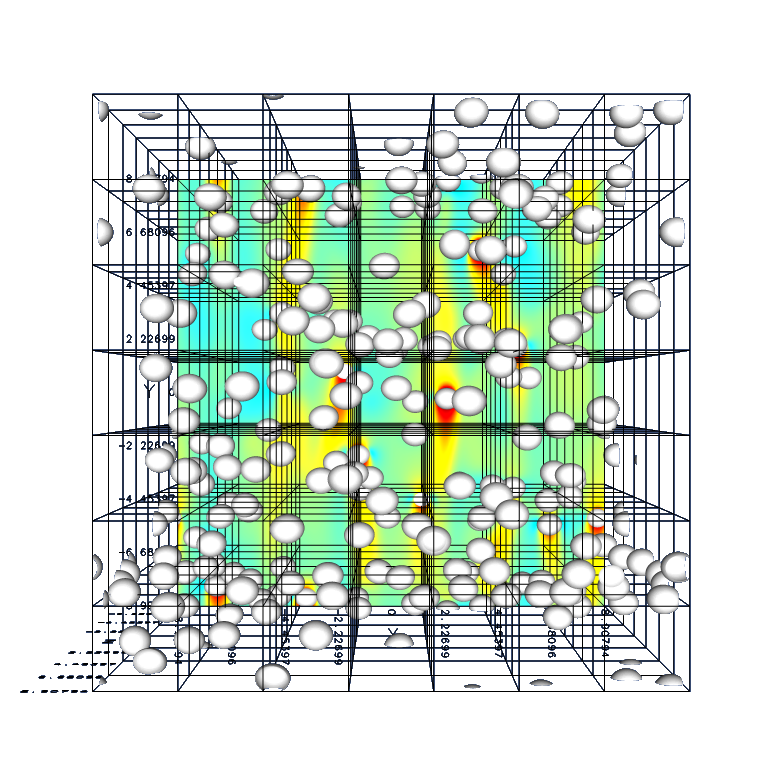
\includegraphics[width =  1.1\textwidth]{image/PHI_01_Ga_75.png}
  \end{columns}
\end{frame}

\section{Drag force}
\section{}
\begin{frame}{Averaged \underline{Mass} and \underline{Momentum} averaged equations }
  \begin{align*}
    &\pddt (\phi_f \rho_f)  
    + \div (
        \phi_f \rho_f\textbf{u}_f
    )
    = 
    0,\\
    &
    \phi_f \rho_f (\pddt + \textbf{u}_f\cdot \grad)\textbf{u}_f
    = 
    \underbrace{\div \bm\sigma^\text{eff}}_\text{Effective stress}
    + \underbrace{\phi_f \rho_f \textbf{g} }_\text{buoyancy}
    \textcolor{cyan}{- \underbrace{\pSavg{{\bm{\sigma}_f^0 \cdot \textbf{n}}}}_\text{Interphase drag force}},
  \end{align*}
  \underline{Effective stress: } 
  \begin{equation*}
    \bm{\sigma}_f^\text{eff}
    =
    - \underbrace{\avg{\chi_f\rho_f\textbf{u}_f'\textbf{u}_f'}}_\text{Reynolds Stress}
    + \underbrace{\phi_f \bm{\sigma}_f}_\text{Mean Newtonian stress}%- n_p \textbf{M}_p
     + \underbrace{ {\pSavg{{\textbf{r}\bm{\sigma}_f^0 \cdot \textbf{n}}}}}_\text{First moment}
     -\underbrace{\div [\ldots]}_\text{higher moments}
  \end{equation*}
\end{frame}


\begin{frame}
  \frametitle{Drag   coefficient : Measurements with the DNS}

\centering    
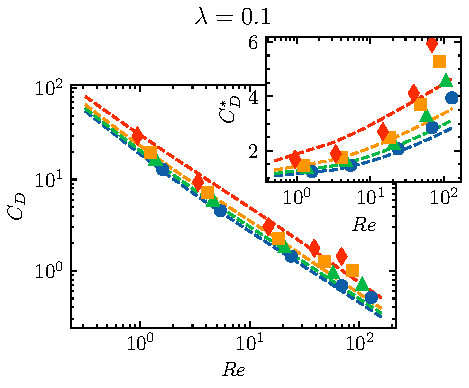
\includegraphics[height = 0.25\textwidth]{image/HOMOGENEOUS_final/CA/Cp_l_0.pdf}
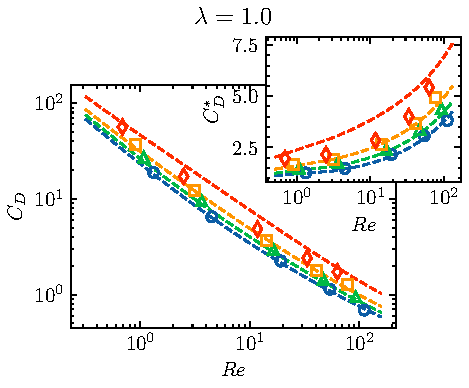
\includegraphics[height = 0.25\textwidth]{image/HOMOGENEOUS_final/CA/Cp_l_1.pdf}
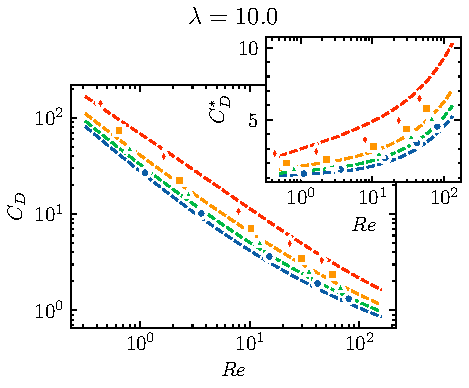
\includegraphics[height = 0.25\textwidth]{image/HOMOGENEOUS_final/CA/Cp_l_10.pdf}
\begin{equation*}
\pSavg{{\bm{\sigma}_f' \cdot \textbf{n}}}
= 
 \frac{1}{2} n_p a^2 \pi \rho_f 
  \underbrace{C_D(Re,\phi,\textcolor{sintefred}{\lambda})  }_\text{Drag force coefficient}
  |\textbf{U}| \textbf{U}
\end{equation*}
\begin{itemize}
    \item $\textbf{U} = \textbf{u}_p - \textbf{u}_f$ Mean relative velocity 
    \item $a$ droplet radius
    \item $n_p$ Number of droplets per unit of volume
\end{itemize}
\end{frame}





\section{First moment}
\section*{}





\begin{frame}{Averaged \underline{Mass} and \underline{Momentum} averaged equations }
  \begin{align*}
    &\pddt (\phi_f \rho_f)  
    + \div (
        \phi_f \rho_f\textbf{u}_f
    )
    = 
    0,\\
    &
    \phi_f \rho_f (\pddt + \textbf{u}_f\cdot \grad)\textbf{u}_f
    = 
    \underbrace{\div \bm\sigma^\text{eff}}_\text{Effective stress}
    + \underbrace{\phi_f \rho_f \textbf{g} }_\text{buoyancy}
    - \underbrace{\pSavg{{\bm{\sigma}_f^0 \cdot \textbf{n}}}}_\text{Interphase drag force},
  \end{align*}
  \underline{Effective stress: } 
  \begin{equation*}
    \bm{\sigma}_f^\text{eff}
    =
    - \underbrace{\avg{\chi_f\rho_f\textbf{u}_f'\textbf{u}_f'}}_\text{Reynolds Stress}
    + \underbrace{\phi_f \bm{\sigma}_f}_\text{Mean Newtonian stress}%- n_p \textbf{M}_p
    \textcolor{cyan}{ + \underbrace{ {\pSavg{{\textbf{r}\bm{\sigma}_f^0 \cdot \textbf{n}}}}}_\text{First moment}}
     -\underbrace{\div [\ldots]}_\text{higher moments}
  \end{equation*}
\end{frame}



\begin{frame}{What is the Stresslet ?}
\begin{equation*}
  \pSavg{\textbf{r}\bm{\sigma}_f^0 \cdot \textbf{n}}
  = 
  \underbrace{\pSavg{(\textbf{r}\bm{\sigma}_f^0 +\bm{\sigma}_f^0 \textbf{r} )\cdot \textbf{n}}}_\text{Symmetric part = Stresslet}
  +
  \bm\epsilon \cdot \underbrace{\pSavg{\textbf{r} \times \bm{\sigma}_f^0 \cdot \textbf{n}}}_\text{Skew-symmetric part $\propto$  Torque}
\end{equation*}

\setbeamercovered{transparent=10}
\only<1>{
  \centering
  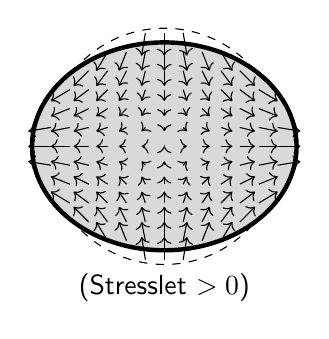
\begin{tikzpicture}[ultra thick,scale=0.6]
    \def\nRows{6}
    \def\nCols{6}
    \draw[dashed,thin] (0,0)circle(2.5);
    \draw[fill=gray!30] (0,0)ellipse(2.8 and 2.2);
    \foreach \x in {-\nRows,...,\nRows} {
        \foreach \y in {-\nCols,...,\nCols} {
            \pgfmathsetmacro\distance{veclen(\x*0.4, \y*0.4)};
            \pgfmathparse{\distance < 2.45 ? "blue" : "white"}
            \edef\colour{\pgfmathresult};
            \ifthenelse{\equal{\colour}{blue}}{                    
                \draw[thin,->](\x*0.4,\y*0.4)--++(0.08*\x,-0.08*\y);
            }
        }
    }
    \node (txt) at (0,-3){(Stresslet $> 0$)};
\end{tikzpicture}
\hspace{1em}
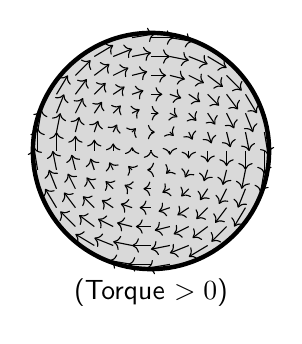
\begin{tikzpicture}[ultra thick,scale=0.6]
    \def\nRows{6}
    \def\nCols{6}
    \draw[fill=gray!30] (0,0)circle(2.5);
    \foreach \x in {-\nRows,...,\nRows} {
        \foreach \y in {-\nCols,...,\nCols} {
            \pgfmathsetmacro\distance{veclen(\x*0.4, \y*0.4)};
            \pgfmathparse{\distance < 2.5 ? "blue" : "white"}
            \edef\colour{\pgfmathresult};
            \ifthenelse{\equal{\colour}{blue}}{                    
                \draw[thin,->](\x*0.4,\y*0.4)--++(0.08*\y,-0.08*\x);
            }
        }
    }
    \node (txt) at (0,-3){(Torque $> 0$)};
\end{tikzpicture}
}
\only<2->{
\uncover<2>{\textbf{Shear dominated flows, Stokes regime: }
\begin{equation*}
  \pSavg{(\textbf{r}\bm{\sigma}_f^0 +\bm{\sigma}_f^0 \textbf{r} )\cdot \textbf{n}}
  = \frac{3}{5}\mu_f \phi \left(\frac{2+5\lambda}{1+\lambda}\right) \left(\grad \textbf{u}_f + ^\dagger \grad \textbf{u}_f\right)
  + \mathcal{O}(\phi^2, Re)
\end{equation*}
Thus, $\frac{3}{5}\phi \left(\frac{2+5\lambda}{1+\lambda}\right)$ it can be considered as an effective viscosity ! 
}

\uncover<3>{\textbf{Droplet in translation, Stokes regime: }
\begin{equation*}
  \pSavg{(\textbf{r}\bm{\sigma}_f^0 +\bm{\sigma}_f^0 \textbf{r} )\cdot \textbf{n}}
  = 0 + \mathcal{O}(\phi Re)
\end{equation*}
So the relative velocity doesn't contribute to the Stresslet  ? 

}

\uncover<4>{
  \textbf{We must consider the effect of finite $Re$  !}
}}
\end{frame}

\begin{frame}
  \frametitle{Reformulation of the first moment  with conditional average}
  
    \begin{equation*}
      \underbrace{\pSavg{{\textbf{r} \bm{\sigma}_f^0 \cdot \textbf{n}}}[\textbf{x},t]}_\text{$N$ droplets in a fluid}
      =
      \underbrace{n_p[\textbf{x},t]
        \intS[]{\textbf{r} \bm\sigma^1 \cdot \textbf{n}}}_\text{
        \href{videos/one_particle.mp4}{One droplet in an effective medium}
        }
    \end{equation*}
  \begin{itemize}
    \item $\bm\sigma^1[\textbf{z}|\textbf{x}]$ Mean stress at \textbf{z} conditioned on the presence of a droplet at $\textbf{x}$. 
  \end{itemize} 
  \vfill
  $\to$ This time we need a result of $\bm\sigma$ accurate at $\mathcal{O}(Re)$. 
\end{frame}

% \begin{frame}
%   {Conditional averaged equation at $\mathcal{O}(\phi)$ and finite $Re$ }
%   \textbf{Navier-Stokes equations}: 
%   \begin{align*}
%     \div \textbf{v} &= 0 \\
%       \mu_f \grad^2 \textbf{v}  
%         - \grad p_f 
%       &\only<1->{ =
%       Re \left[
%         \pddt \textbf{v}
%         + \textbf{v}\cdot \grad\textbf{v} 
%         -  \textbf{v}\cdot \grad\textbf{U} 
%         -  \textbf{U}\cdot \grad\textbf{v}
%     \right]}
%     % \uncover<2->{\\ &= Re\textbf{f}} 
% \end{align*}
% \textbf{Boundary conditions}:
% \begin{align*}  
%   \textbf{v}\cdot \textbf{n} &= \textbf{U} \cdot \textbf{n} 
%   && 
%   r = 1 \\
%   \textbf{v} &= 0 && r \to \infty
% \end{align*}

% \only<1>{
%   \begin{itemize}
%   \item $\textbf{v}$ Disturbance velocity field generated by a translating droplet. 
%   \item $\textbf{U} =\textbf{u}_p - \textbf{u}_f$ relative background velocity. 
%   % \item<2-> $\textbf{f}$ Inertial contribution. 
% \end{itemize}
% $\to$ Similar to \citet{maxey1983equation} \& \citet{gatignol1983faxen}'s equations !
% }
% \only<2>{Only $\boxed{\intS[]{\textbf{r} \bm\sigma \cdot \textbf{n}}}$ is needed not $\textbf{v}$ ! $\to$ \textbf{Reciprocal theorem} \citep{stone2001inertial}}
% \end{frame}



% \begin{frame}
%   \frametitle{How to derive the reciprocal theorem ? }
%   % \setbeamercovered{transparent=10}
%   Let  $\hat{\textbf{v}}$ be a \textbf{known solution} of the Stokes equations: 
% \vfill
%   {\Huge Step \only<1>{1}\only<2>{2}\only<3->{3}:
%   }
%   \begin{equation*}
%     \uncover<3->{\int_{V_f}\left\{ }
%     \fbox{Equation of \textbf{v}} \cdot \hat{\textbf{v}} 
%     \uncover<2->{
%       - \fbox{Equation of $\hat{\textbf{v}}$} \cdot  \textbf{v} 
%       }
%     \uncover<3->{\right\}dV}
%     \uncover<4>{= 0}
%   \end{equation*}
% \end{frame}

\begin{frame}
  \frametitle{Stresslet due to the relative motion of the drops}
\setbeamercovered{transparent=15}


  \begin{equation*}
    \frac{a}{\mu_f U}
    % \left[
        \pSavg{\textbf{r}\bm{\sigma}_f^0 \cdot \textbf{n}}
        % - \pOavg{(2 \mu_f \textbf{e}_d^0 - p_f\textbf{I})}
        % \right]
        % \\
    =
    \phi Re C_1
    [
      \textbf{UU} - \frac{1}{3}(U^2)\textbf{I} 
      ]
      + Re \phi C_2 (U^2) \textbf{I}
      % + \phi p_f \textbf{I}
  \end{equation*} 
\begin{align*}
    C_1  =  -\frac{63 \lambda^{3} + 150 \lambda^{2} + 112 \lambda + 28}{80 \left(\lambda + 1\right)^{3}}
    &&
    C_2  = \frac{3\lambda^2 + 6\lambda + 4}{48(\lambda +1 )^2}
  \end{align*}
  
  \begin{itemize}
    \item \textbf{U}=$\textbf{u}_p-\textbf{u}_f$ Mean relative velocity between phases
  \end{itemize}
  $\to$ Rising droplets deform when $Re > 0$ due to the non-zero Stresslet !. 

\end{frame}

\section{Reynolds stress}
\section*{}


\begin{frame}{Averaged \underline{Mass} and \underline{Momentum} averaged equations }

  \begin{align*}
    &\pddt (\phi_f \rho_f)  
    + \div (
        \phi_f \rho_f\textbf{u}_f
    )
    = 
    0,\\
    &
    \phi_f \rho_f (\pddt + \textbf{u}_f\cdot \grad)\textbf{u}_f
    = 
    \underbrace{\div \bm\sigma^\text{eff}}_\text{Effective stress}
    + \underbrace{\phi_f \rho_f \textbf{g} }_\text{buoyancy}
    - \underbrace{\pSavg{{\bm{\sigma}_f^0 \cdot \textbf{n}}}}_\text{Interphase drag force},
  \end{align*}
  \underline{Effective stress: } 
  \begin{equation*}
    \bm{\sigma}_f^\text{eff}
    =
    \textcolor{cyan}{- \underbrace{\avg{\chi_f\rho_f\textbf{u}_f'\textbf{u}_f'}}_\text{Reynolds Stress}}
    + \underbrace{\phi_f \bm{\sigma}_f}_\text{Mean Newtonian stress}%- n_p \textbf{M}_p
     + \underbrace{ {\pSavg{{\textbf{r}\bm{\sigma}_f^0 \cdot \textbf{n}}}}}_\text{First moment}
     -\underbrace{\div [\ldots]}_\text{higher moments}
  \end{equation*}
\end{frame}



\begin{frame}{Objectives and assumptions}
  \begin{equation*}
     \avg{\chi_f \textbf{u}_f'\textbf{u}_f'}
     = 
     \text{Particle induced turbulence}
     + \text{
      \only<1>{Single phase turbulence}
      \only<2>{\cancel{Single phase turbulence}}
      }
  \end{equation*}
  \uncover<2>{
    \begin{columns}
      \column{0.6\textwidth}
      \begin{itemize}
        \item 
        Focus on the \textbf{Particle induced turbulence}. 
        \item Assuming : 
        \begin{itemize}
          \item Negligible inertia (\textbf{Stokes} regime)
          \item Dilute regime.
          \item Mono-disperse suspension of droplets . 
        \end{itemize}
      \end{itemize}
      \column{0.4\textwidth}
      \centering
      Streamlines around a rising droplet: 
      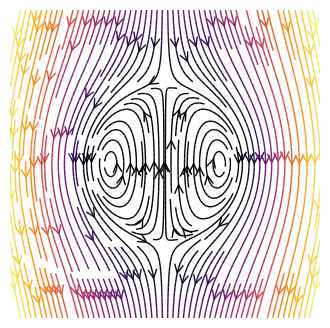
\includegraphics[width=0.8\textwidth]{image/Rising_Stokes.png}
    \end{columns}
    }
\end{frame}

\begin{frame}
  {Nearest Particle Statistics (NPS) approach \citep{zhang2021ensemble}}
  % Using the relation between ensemble average $\avg{\ldots}$ and NPS average we obtain :
  \setbeamercovered{transparent=10}

  \begin{equation*}
    \avg{\chi_f \textbf{u}'_f\textbf{u}'_f}[\textbf{x},t]
    = 
    \underbrace{
      \phi_f
      \int 
      \textbf{v}^\text{nst}_f
      \textbf{v}^\text{nst}_f 
      P_\text{nst}d\textbf{r} 
    }_\text{
      \href{videos/nst_particles.mp4}{
        \only<1>{Averaged wake contribution}
        \only<2->{$\propto \phi^{2/3}$}
    }}
    \uncover<3->{+ \underbrace{ 
      \int \avg{\chi_f \textbf{v}_f''\textbf{v}_f'' \delta_i h_i }  d\textbf{r}
    % P_{nst}(\textbf{x},t,\textbf{r}) d\textbf{r}
    }_\text{
      \only<3>{All others contributions}
      % \only<4>{$\propto \phi^{2/3} !!!! $}
      }
    }
  \end{equation*}

\begin{itemize}
  \item $P_\text{nst}[\textbf{r}+\textbf{x}|\textbf{x}]$ is the probability of finding a nearest particle at $\textbf{r}+\textbf{x}$ knowing \textbf{x} is occupied by the continuous phase.   
  \item $\textbf{v}_f^\text{nst}[\textbf{r}+\textbf{x},\textbf{x}]$ disturbance velocity evaluated at \textbf{x}, averaged on every configuration where the nearest particle to the point \textbf{x} is located at $\textbf{r}+\textbf{x}$. 
  \item<3-> $\textbf{v}''_f = \textbf{u}^0_f - \textbf{u}^\text{nst}_f$ fluctuating values of the local velocity $\textbf{u}_f^0$ (non-averaged) around $\textbf{u}_f^\text{nst}$.
\end{itemize}
\end{frame}

\begin{frame}
  \frametitle{Summary of the results}
Based on \textbf{theoretical analysis} and \textbf{measurements} from the DNS:

\begin{align*}
  \avg{\chi_f \textbf{u}_f'\textbf{u}_f'}
  = 
  C_1^{Re} \left[
      \textbf{U}\textbf{U}
       - \frac{1}{3}(
        \textbf{U}\cdot \textbf{U}
       )\textbf{I}
  \right]
  + 
  C_2^{Re}  (\textbf{U}\cdot \textbf{U})\textbf{I}
\end{align*}

\begin{align*}
  C_1^{Re}(Re,\textcolor{sintefred}{\phi},\lambda)
  &=
  \underbrace{\frac{(2+3\lambda)^2}{(\lambda+1)^2}
  \textcolor{sintefred}{\phi^{2/3}}}_\text{Theoritical analysis}
  \times 
  \underbrace{f_1(Re)}_\text{Empirical factor}
  \uncover<2>{\\
  C_2^{Re}(Re,\phi,\lambda)
  &=
  C_1^{Re}(Re,\phi,\lambda)
  \times 
  f_2(Re)}
\end{align*}

\begin{itemize}
  \item $\textbf{U} = \textbf{u}_p - \textbf{u}_f$ relative velocity. 
\end{itemize}
$\to$ The $\textcolor{sintefred}{\phi^{2/3}}$ tends is valid across $Ga = [5,100]$. 
\end{frame}

\section{Effective stress}
\section*{}

\begin{frame}
  \frametitle{Effective stress in homogeneous buoyant emulsions }
  \setbeamercovered{transparent=15}
    \begin{equation*}
      \phi_f \rho_f (\pddt + \textbf{u}_f\cdot \grad)\textbf{u}_f
      = 
      \div \bm\sigma^\text{eff}
      + \phi_f \rho_f \textbf{g} 
      - \pSavg{{\bm{\sigma}_f^0 \cdot \textbf{n}}}
  \end{equation*}
  \underline{Assuming $\grad \textbf{u}_f = 0$ :}
  \begin{align*}
    \frac{a }{\mu_f U}\bm{\sigma}^\text{eff}_f 
    &=
    -  \avg{\chi_f\rho_f\textbf{u}_f'\textbf{u}_f'}
    +  \phi_f \bm{\sigma}_f
    +  \pSavg{{\textbf{r}\bm{\sigma}_f^0 \cdot \textbf{n}}}
    \text{}{+ \div [\ldots]}
    \\
    \uncover<2>{&= 
    \left[ p_f + Re \phi  (C^{Re}_2 - C_2)(\textbf{U}\cdot \textbf{U}) \right]\textbf{I} 
    + Re \phi (C^{Re}_1 - C_1)\left[
            \textbf{U}
            - \frac{1}{3}(\textbf{U}\cdot \textbf{U})\textbf{I}
    \right]}
    % + \mathcal{O}(Re^{3/2},\phi^2).
    \label{eq:stress_closed}
\end{align*} 
\uncover<2>{
\textbf{Which one is more important $C$ or $C^{Re}$ ?  }
}

\end{frame}

% \begin{frame}
%   \frametitle{How to compute the first moment within the DNS ?}

%   \underline{Steady state} first moment of momentum equation:
%   \begin{multline*}
%     \pSavg[i]{\textbf{r}\bm\sigma_f^0\cdot \textbf{n}}
%     = 
%     \underbrace{- \pOavg[i]{\rho_d \textbf{w}_d^0  \textbf{w}_d^0 }
%     + \pOavg[i]{\bm\sigma_d^0}}_\text{volume integrals}\\
%     +  \underbrace{\gamma \pSavg[i]{(\textbf{I} - \textbf{nn})}}_\text{Geometry of the surface}
% \end{multline*}

% \uncover<2>{$\to$ We are thus able to meusure $C_1$ (and $C^{Re}_1$) from DNS !}
% \end{frame}

\begin{frame}{Comparison with simulations results}
  \begin{figure}[h!]
    \centering
    \uncover<2>{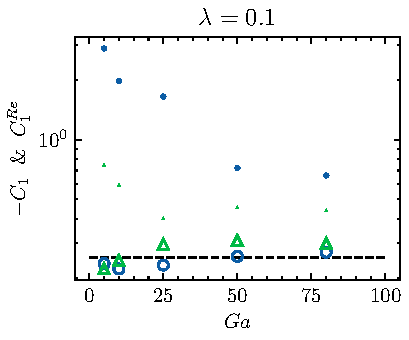
\includegraphics[height = 0.25\textwidth]{image/HOMOGENEOUS_final/PA/Sdev_diapo_l_1.pdf}}
    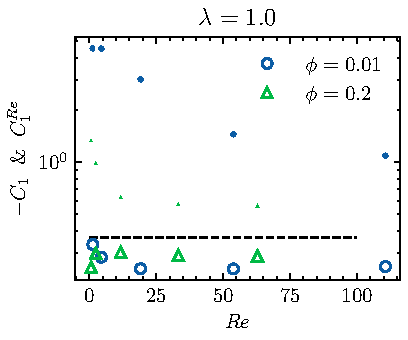
\includegraphics[height = 0.25\textwidth]{image/HOMOGENEOUS_final/PA/Sdev_diapo_l_10.pdf}
    \uncover<2>{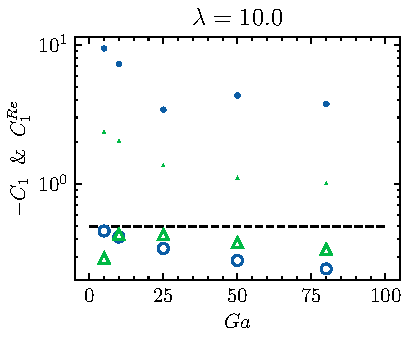
\includegraphics[height = 0.25\textwidth]{image/HOMOGENEOUS_final/PA/Sdev_diapo_l_100.pdf}}
    \caption{
      (Hollow symbols) \underline{Stresslet}: $C_1$. 
      (Filled symbols) \underline{Reynolds stress} $C_1^{Re}$. 
     }
\end{figure}

\uncover<2>{
\textbf{In dense regime the Stresslet may not be negligible !}
}


\end{frame}



\section{Conclusion}
\section*{}

\begin{frame}
  \frametitle{What have we learned ? }
  \setbeamercovered{transparent=10}

\textbf{Methodology: }
  \begin{itemize}
    \item How to derive ensemble averaged equations. 
    \item How to relate \underline{closure terms} to the \underline{closure problems}, and how to solve them (singularity method, reciprocal theorem or DNS).
    DNS: \url{http://basilisk.fr/sandbox/fintzin/Rising-suspension/RS.c}
  \end{itemize}

  \uncover<2>{
\textbf{Physics :}
\begin{itemize}
  \item Drag force: $\sim U^2 C_D(Re, \phi,\textcolor{sintefred}{\lambda})$.
  \item Reynolds stress: $\sim U^2 \phi^{2/3}$.
  \item Stresslet: $\sim U^2 \phi$.
  \item And Reynolds stress $\approx$ Stresslet for high $\phi$ and Reynolds stress $\ll$ Stresslet for $\phi \ll 1$.
 \end{itemize}
}


\end{frame}
\begin{frame}
  \frametitle{Buoyancy driven emulsion rheology}
  \centering\underline{Continuous phase mass and momentum equation:}
  \begin{equation*}
    \pddt \phi_f + \div (\textbf{u}_f \phi_f) = 0
  \end{equation*}
  \begin{equation*}
    % \pddt \phi_f + \div (\textbf{u}_f \phi_f) &= 0\\ 
      \rho_f (\pddt 
    + \textbf{u}_f \cdot \grad)
    \textbf{u}_f
    = 
    \div\bm\Sigma_f
    % \underbrace{\div\bm\Sigma_f}_\text{Newtonian stress}
    + \rho_f \textbf{g}
    \only<2->{\textcolor{sintefcyan}{-\underbrace{\frac{3\rho_f}{8a} \frac{\phi C_D(Re,\phi, \lambda) }{1-\phi}   \times \textbf{U} |\textbf{U}|}_\text{Drag force}}}
    \only<3>{\textcolor{sintefred}{+\underbrace{\frac{1}{1-\phi} \div  \bm{\sigma}_f^{\text{eff}}}_\text{Effective stress}}}
  \end{equation*}

  \centering\underline{Constitutive laws:}

\begin{equation*}
    \bm\Sigma_f 
    = 
    - p_f \textbf{I}
    + 2\mu_f \left[\grad \textbf{u}_f + (\grad \textbf{u}_f)^\dagger\right]
\end{equation*}

\uncover<3>{
\begin{equation*}
\textcolor{sintefred}{
    \bm{\sigma}^{\text{eff}}_f 
    = \underbrace{C_E(Re,\phi,\lambda) \mu_f [\grad \textbf{u}_f +  (\grad \textbf{u}_f)^\dagger ] }_\text{``Einstein viscosity'' \& Single phase Turbulence}
    + 
    \underbrace{
      C_1(\phi,\lambda,Re)\textbf{UU}
    + C_2(\phi,\lambda,Re)U^2 \textbf{I}}_\text{Mean particle Induced Turbulence (PIT) \& Stresslet}
}
\end{equation*}
}

\end{frame}


\begin{frame}
  \frametitle{Applications}
\textbf{Domain of validity of the closures laws}:
  \begin{itemize}
    \item Dispersed two-phase flows ($\phi < 0.2$)
    \item Small droplets or bubbles ($Bo < 1$ and $Re < 100$)
    \item Buoyancy driven flows
  \end{itemize}
\vfill
  \textbf{Target processes:  }
  \begin{itemize}
    \item Liquid-Liquid separation
    \item Flotation (clean waste water)
    \item Transport of tiny particles in liquid
  \end{itemize}

\end{frame}


\begin{frame}
  \centering
  {\Huge\textbf{Perspectives ? }}

  \begin{itemize}
    \item Dispersed phase equations ? (Center of mass velocity variance ? )
    \item How to measure $C_1$, $C_2$ with experiments  ?
    \item Hyperbolic system of equations ? With effective stress $\propto U^2$ ?
    \item Are the proposed closures laws consistent with thermodynamics constrains ?
  \end{itemize}

\end{frame}
\backmatter

\begin{frame}
  \footnotesize

  \bibliography{Bib/bib_bulles.bib}

\end{frame}


\begin{frame}
  {Reciprocal theorem: final expression }
\small
  % Applying the reciprocal theorem between $\textbf{v}$ and a \underline{known} test problem: $\hat{\textbf{v}}$, gives, 
\begin{align*}
  \underbrace{
    \intS[]{\hat{\textbf{U}} \cdot  \bm\sigma \cdot \textbf{n}}
    - \intO[d]{
        \grad \textbf{v} :\grad \hat{\textbf{U}} 
   }
  }_\text{What we are looking for}
    &=
    \intS[]{\textbf{U}\cdot \hat{\bm\sigma}\cdot \textbf{n}}
    + (\lambda - 1)\intS[]{
      \textbf{U}\cdot (\grad \hat{\textbf{U}}+ ^\dagger \grad \hat{\textbf{U}})\cdot \textbf{n}
    }\\
    &- \lambda \intO[d]{\grad \hat{\textbf{v}}:\grad \textbf{U}} 
    - 
    \only<1>{Re \zeta \intO[d]{(\hat{\textbf{v}} - \hat{\textbf{U}}) \cdot \textbf{f}}}
    \only<2>{\textcolor{sintefred}{Re \zeta \intO[d]{(\hat{\textbf{v}} - \hat{\textbf{U}}) \cdot \textbf{f}}}}
    \\
    &
    -
    \only<1>{Re \intOf{\hat{\textbf{v}} \cdot  \textbf{f}}}
    \only<2>{\textcolor{sintefred}{Re \intOf{\hat{\textbf{v}} \cdot  \textbf{f}}}}
\end{align*}

\only<1>{
\begin{itemize}
  \item $V_f$ denote the domain outside the test droplet
  \item $V_d$ denote the domain inside the test droplet
\end{itemize}
\vfill
$\to$ \textbf{Methodology from \citet{stone2001inertial} (solid spheres)}
}
\uncover<2>{
  \underline{Known fields:}
  \begin{itemize}
    \item Boundary conditions: $\hat{\textbf{U}}, \textbf{U}$.  
    \item Test solution $\hat{\textbf{v}},\hat{\bm\sigma}$
  \end{itemize}
  \underline{Unknown fields:}
  \begin{itemize}
    \item \textcolor{sintefred}{Inertial term: \textbf{f}}
  \end{itemize}
}
\end{frame}


\begin{frame}
  \frametitle{Regular expansion in $Re$ }

  Assuming small but finite $Re$ : $\textbf{f} = \textbf{f}^{(0)} + Re  \textbf{f}^{(1)} + Re^2  \textbf{f}^{(2)} + \ldots$. 

  
  \begin{equation*}
    \textbf{f}^{(0)}
    =
        \pddt \textbf{v}^{(0)}
        + \textbf{v}^{(0)}\cdot \grad\textbf{v}^{(0)} 
        +  \textbf{v}^{(0)}\cdot \grad\textbf{U} 
        +  \textbf{U}\cdot \grad\textbf{v}^{(0)}
  \end{equation*}

  $\to$ $\textbf{v}^{(0)}$ is governed by the Stokes equation this is thus a known field ! 
  \uncover<2>{
  \begin{equation}
      Re \intOf{\hat{\textbf{v}} \cdot  \textbf{f}}
      =
      Re \intOf{\hat{\textbf{v}} \cdot  \textbf{f}^{(0)}}
      + \mathcal{O}(Re^2)
    \end{equation}
    }
\end{frame}
\begin{frame}
  \frametitle{Example: Drag force on a droplet in arbitrary Stokes flow}
  \begin{itemize}
    \item $\textbf{v}$ Arbitrary quadratic stokes flow ($Re=0$).  
    \item $\hat{\textbf{v}} = $ disturbance velocity field of a droplet translating in uniform flow. 
  \end{itemize}

  \begin{equation}
    \intS{\cdot  \bm\sigma_f \cdot \textbf{n}}
    =
    a 2\pi \left(
      \frac{3\lambda +2 }{\lambda +1} 
    \right) \textbf{U}
    + 
    a^3 \pi \frac{\lambda}{\lambda +1}
    \grad^2 \textbf{U}
  \end{equation}
\end{frame}


\begin{frame}
  \frametitle{What about the remaining term ? }

  \begin{equation*}
    \avg{\chi_f \textbf{u}'_f\textbf{u}'_f}[\textbf{x},t]
    = \phi_f
    \underbrace{\int 
      \textbf{v}^\text{nst}_f
      \textbf{v}^\text{nst}_f 
      P_\text{nst}d\textbf{r} 
    }_{\sim C \phi^{2/3} }
    + \underbrace{ 
      \int \avg{\delta_i h_i \chi_f \textbf{v}_f''\textbf{v}_f''}  d\textbf{r}
    % P_{nst}(\textbf{x},t,\textbf{r}) d\textbf{r}
    }_\text{What is that supposed to mean ?}
  \end{equation*}
\uncover<2->{
\begin{multline*}
    \int \avg{\delta_i h_i \chi_f \textbf{v}_f''\textbf{v}_f''}  d\textbf{r}
    = 
    \underbrace{\int 
    \textbf{v}^{(\text{2-nst})}_f
    \textbf{v}^{(\text{2-nst})}_f 
    P_\text{2-nst}
    d\textbf{r}^2}_{\sim \phi^{2/3}}
    +  
    \uncover<3->{\underbrace{\int 
    \textbf{v}^{(\text{3-nst})}_f
    \textbf{v}^{(\text{3-nst})}_f 
    P_\text{3-nst}
    d\textbf{r}^3}_{\phi^{2/3}}
    }\\
    \uncover<4->{+\ldots\underbrace{\int 
    \textbf{v}^{(\text{N-nst})}_f
    \textbf{v}^{(\text{N-nst})}_f 
    P_\text{N}
    d\textbf{r}^N}_{  \sim \phi^{2/3}}}
\end{multline*}
}
  % \only<2-3>{\vspace{-2cm}
  %   \begin{itemize}
  %     \item $\textbf{u}_f^2$ Velocity averaged on every configuration were the nearest neighbor is at $\textbf{r}$ and the $2^{nd}$ nearest neighbor at $\textbf{r}_2$. 
  %     \item $\textbf{v}_f^2 = \textbf{u}_f^2 - \textbf{u}_f^\text{nst}$. 
  %   \end{itemize}
  %   }

\only<5>{
  $\rightarrow$ $\lim_{N \to \infty} \avg{\chi_f \textbf{u}'_f\textbf{u}'_f} = \infty $
  (Caflisch and Luke (1985))

  $\to$ We only consider the first intergral. 
}
\end{frame}

\end{document}

\begin{frame}
  {Solution to the first integral}
  \begin{align*}
    \int\textbf{v}^\text{nst}_f
    \textbf{v}^\text{nst}_f 
    P_\text{nst} d\textbf{r} 
    = 
    \underbrace{C_1^{(Re= 0)} \left[
        \textbf{U}\textbf{U}
        % + \pavg{\textbf{u}_i'\textbf{u}_i'}/n_p
         - \frac{1}{3}(
          \textbf{U}\cdot \textbf{U}
        %  +2k_p
         )\textbf{I}
    \right]}_\text{deviatoric part}
    + 
    \underbrace{ C_2^{(Re=0)}  (\textbf{U}\cdot \textbf{U}
    % +2k_p
    )\textbf{I}}_\text{Isotropic part}
\end{align*}
\begin{align*}
  C_1^{(Re=0)} =
  \frac{27}{10}
  C_2^{(Re=0)}
  &&  C_2^{(Re=0)} = \frac{(2+3\lambda)^2 \Gamma(\frac{1}{3})}{24(\lambda+1)^2}\textcolor{sintefred}{\phi^{2/3} }
\end{align*}
\uncover<2>{
  \textbf{Assumption:} 
  \begin{equation*}
    \avg{\chi_f \textbf{u}'_f \textbf{u}'_f} / \phi_f= 
    \int\textbf{u}^\text{nst}_f
    \textbf{u}^\text{nst}_f 
    P_\text{nst}(\textbf{r}|\textbf{x}) d\textbf{r} 
    + \underbrace{ 
      \int \avg{\delta_i h_i \chi_f \textbf{v}_f''\textbf{v}_f''}  d\textbf{r}
      % P_{nst}(\textbf{x},t,\textbf{r}) d\textbf{r}
      }_\text{What is that supposed to mean ?} 
  \end{equation*}  
}
\end{frame}








\begin{frame}
  \frametitle{Comparison with DNS results and experiments}
  \begin{figure}[h!]
    \centering    
    % 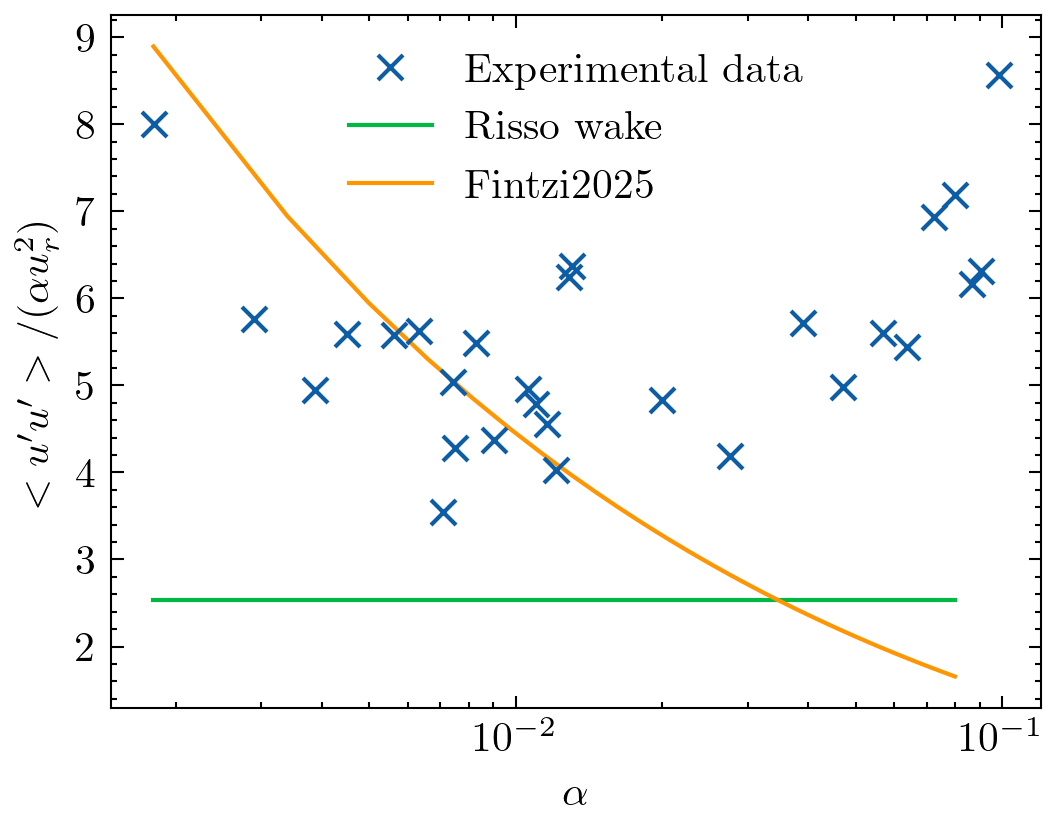
\includegraphics[height = 0.25\textwidth]{image/upupexp.png}
    \uncover<2>{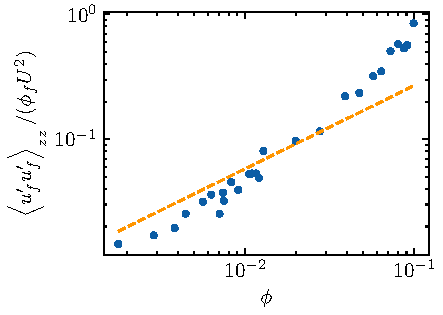
\includegraphics[height = 0.20\textwidth]{image/HOMOGENEOUS_final/CA/cartellier.pdf}}
    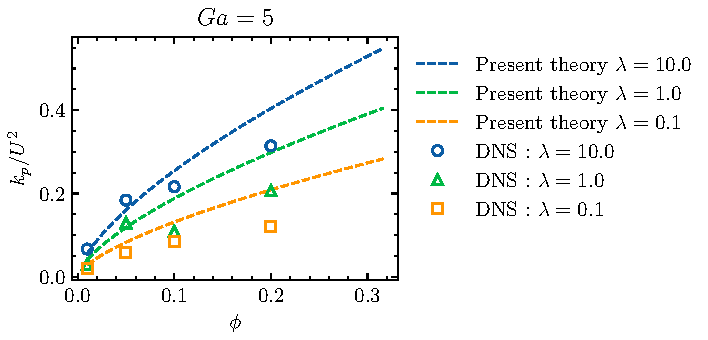
\includegraphics[height = 0.20\textwidth]{image/HOMOGENEOUS_final/CA/UUyy_Ga_5.pdf}
    \caption{
      %  Dimensionless vertical component of the Reynolds stress :
      (right) comparison with DNS for two viscosity ratio $\lambda =1,10$ and $Re \approx 1$ DNS. 
     \uncover<2>{  (left) Comparison with the rising bubbles experiment of Cartellier (2009) with $Re \approx 10$. }
    }
\end{figure}  
\begin{itemize}
  \item Good trends in terms of $\sim \phi^{2/3}$ and $\lambda$.  
  \item Quantitative agreement for $\phi < 0.01$.  
\end{itemize}
\end{frame}

\begin{frame}
  \frametitle{Extension to finite inertial numbers}
  \begin{figure}
    \centering
    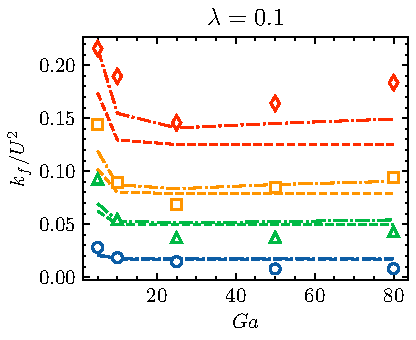
\includegraphics[height = 0.25\textwidth]{image/HOMOGENEOUS_final/CA/KF2_l_0.pdf}
    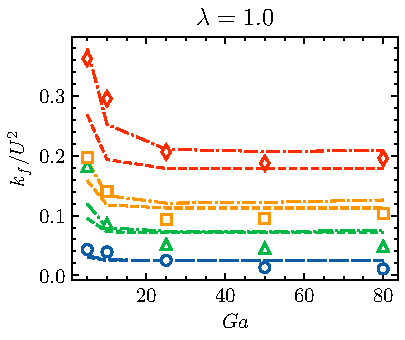
\includegraphics[height = 0.25\textwidth]{image/HOMOGENEOUS_final/CA/KF2_l_1.pdf}
    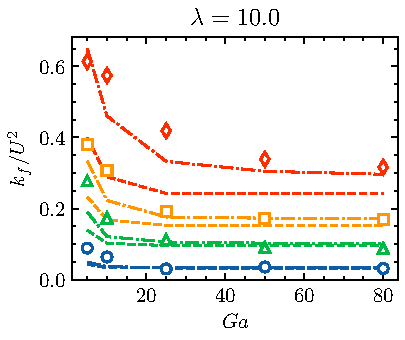
\includegraphics[height = 0.25\textwidth]{image/HOMOGENEOUS_final/CA/KF2_l_10.pdf}
    \caption{\footnotesize
      Continuous phase pseudo turbulent energy, $k_f/U^2 = \avg{\chi_f \textbf{u}_f \cdot \textbf{u}_f}$. 
    % (left) $\lambda = 0.1$
    % (middle) $\lambda = 1$
    % (right) $\lambda = 10$
    (Symbols) DNS results. 
    ($\pmb\bigcirc$) $\phi = 0.01$; ($\pmb\triangle$) $ \phi = 0.05$; ($\pmb\square$) $\phi = 0.1$ ($\pmb\lozenge$) $\phi = 0.2$.
    % (dot-dashed lines) Semi-empirical formula (\ref{eq:semi_empirical}) \underline{including} the results of the DNS for the particle phase velocity fluctuations. 
    % (dashed lines) Semi-empirical formula (\ref{eq:semi_empirical}) \underline{excluding} the particle phase velocity fluctuations. 
    }
    \label{fig:kf}
\end{figure}
\begin{equation}
  C_2^{Re}
  = 
  \underbrace{ C_2^{(Re=0)}}_\text{Theoritical solution}
  \underbrace{\frac{1}{2}\left(e^{-Re} +1\right)}_{\text{empirical factor}}.
  \label{eq:semi_empirical}
\end{equation}

\end{frame}


\begin{frame}
  \frametitle{Comparison with laboratory and numerical experiments }

  \begin{figure}
    \centering
    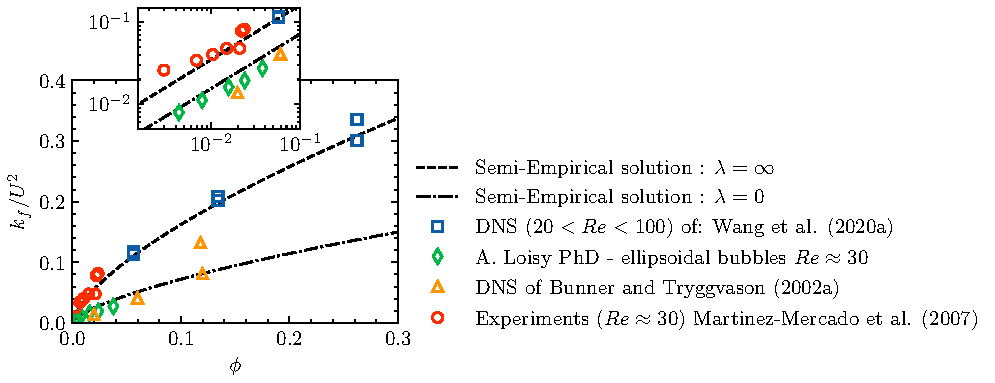
\includegraphics[height = 0.35\textwidth]{image/HOMOGENEOUS_final/CA/KFliterature_diapo.pdf}
\end{figure}
\end{frame}




\begin{frame}
  \frametitle{Reciprocal theorem: test solution in Stokes regime}

  \begin{columns}
    \column{0.7\textwidth}
    \textbf{Stokes equations}: 
    \begin{align*}
      \div \hat{\textbf{v}} &= 0 \\
      \mu_f \grad^2 \hat{\textbf{v}}  
      - \grad \hat{p}_f 
      &= 0 
  \end{align*}
\textbf{Boundary conditions}:
\begin{align*}  
 \hat{\textbf{v}}\cdot \textbf{n} &= [\hat{ \textbf{U}} + \textbf{r}\cdot \grad \hat{\textbf{U}}]\cdot \textbf{n} 
  && 
  r = 1 \\
 \hat{\textbf{v}} &= 0 && r \to \infty\\
\end{align*}

\column{0.3\textwidth}
% \hspace{-3cm}
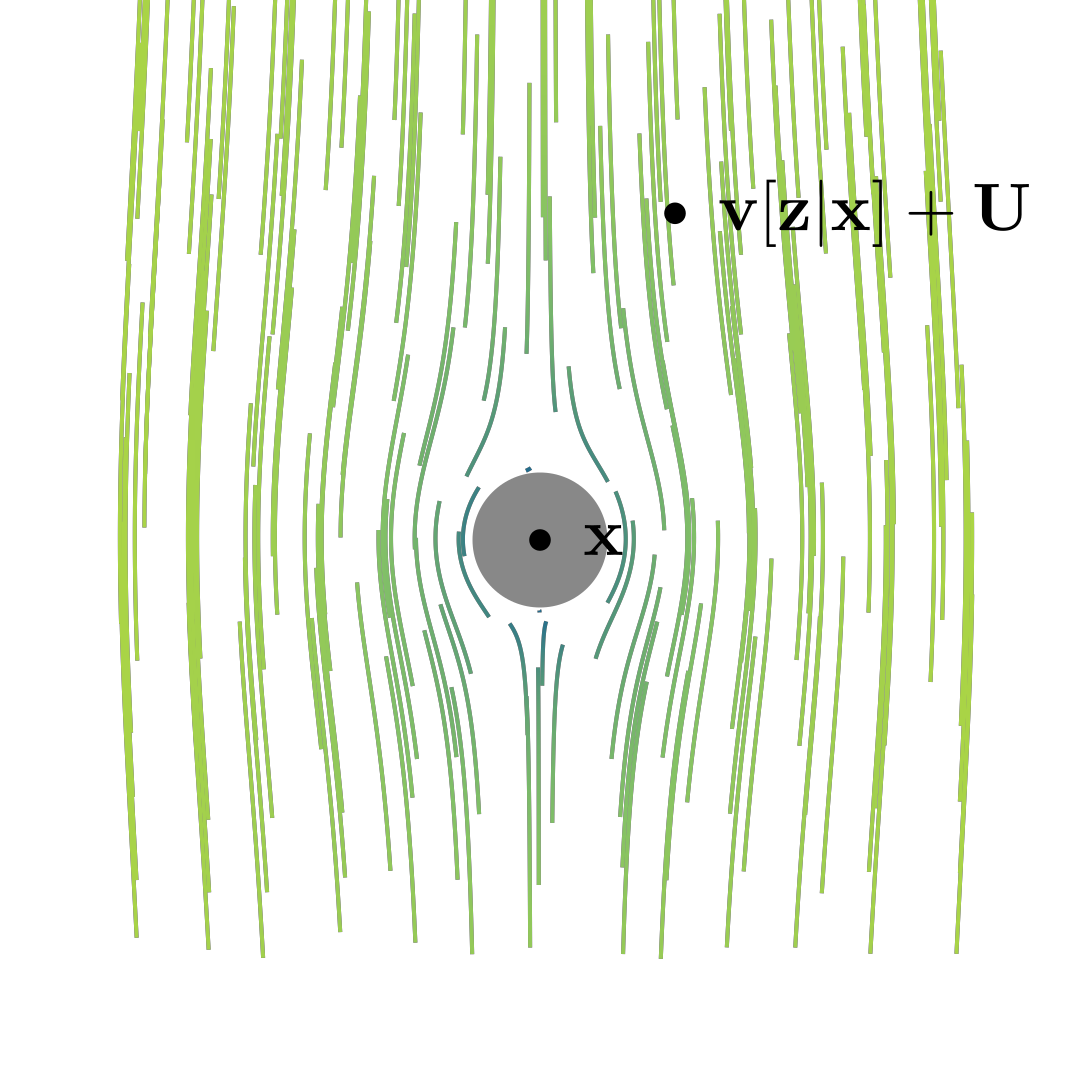
\includegraphics[width = \textwidth]{image/Streamlines_trans.png}
\end{columns}

\uncover<2>{
\textbf{Solution:}
    \begin{equation*}
    \boxed{
    \hat{\textbf{u}}
    =
    \mathcal{U}(\textbf{z}-\textbf{r})\cdot \hat{\textbf{U}}
    + \mathcal{E}(\textbf{z}-\textbf{r}) : \grad\hat{\textbf{U}}
    }
  \end{equation*}
}

\end{frame}

\begin{frame}
  \frametitle{Drag coefficient : semi-empirical model}
    \begin{equation*}
C_D(Re,\phi,\textcolor{sintefred}{\lambda})
    = 
  \only<1>{\underbrace{
    \frac{  \textcolor{sintefred}{\lambda}   C_D^\text{Sol}(Re)+ C_D^\text{Bub}(Re)}
    {1+\textcolor{sintefred}{\lambda}} 
    }_\text{Isolated drag force correlation}}
  \only<2->{
    \frac{  \textcolor{sintefred}{\lambda}   C_D^\text{Sol}(Re)+ C_D^\text{Bub}(Re)}
    {1+\textcolor{sintefred}{\lambda}} 
    }
    \times
    \only<1>{f_\phi(\phi, Re,\textcolor{sintefred}{\lambda})}
    \only<2->{\underbrace{f_\phi(\phi, Re,\textcolor{sintefred}{\lambda})}_\text{Swarm coefficient}}
  \end{equation*}
% \vfill
\only<1>{
  \begin{itemize}
    % \item Creation of a new model which takes in account the viscosity ratio : \textcolor{sintefred}{$\lambda$}. 
    \item $C_D^\text{Sol}$ Drag force coefficient on an isolated \underline{solid sphere} \citep{schiller1933}
    \item $C_D^\text{Bub}$ Drag force coefficient on a \underline{shear-free bubble} \citep{mei1994}
    \item Geometric mean: \citet{magnaudet1997forces} 
  \end{itemize}
  }

\uncover<2->{
\begin{equation*}
  f_\phi(\phi, Re,\textcolor{sintefred}{\lambda})
  =[
    \underbrace{(1-\phi)^{2-n}}_\text{Low Reynolds behavior}
    + 
    \underbrace{Re (1-\phi)^{3-2n}}_\text{High Reynolds behavior}
  ] \frac{1}{1 + Re}
\end{equation*}

\uncover<3>{
  Richardson-Zaki exponent: 
  \begin{equation*}
    n(\textcolor{sintefred}{\lambda},Re) = \frac{\frac{3}{2} \frac{2+3\textcolor{sintefred}{\lambda}}{\textcolor{sintefred}{\lambda}+1} + 2.4 \cdot 0.048 \cdot  Re^{0.75}}{1+0.048 \cdot Re^{0.75}}. 
  \end{equation*}
  }
$\to$ We only included one empirical constant 
}

\end{frame}


\section{Characterization of the microstructure}
\section*{}

% \begin{frame}
%   \frametitle{Motivation for studying microstructure}

%   Study of the microstructure  $=$ analysis of the various arrangements and relative motion that droplets can adopt within
%   dispersed buoyant emulsions. 

%   Motivation: 
%   \begin{enumerate}
%     \item Obtain a better physical understanding of what is acctually happening at the local level
%     \item Coalescence Kernels in Population balence equation
%     \item 
%   \end{enumerate}

% \end{frame}

\begin{frame}
  \frametitle{How to describe pair interactions and microstructure?}
  % To better model the film drainage problem we need a clear understanding of How the interactions between droplets works. 
  
  \textbf{Nearest Particule Statistics (Duan Z. Zhang, JFM, 2021): }
  \begin{definition}
    \begin{itemize}
      % \item Let $\mathscr{C} =\left\{\textbf{x}_1, \textbf{r}, \textbf{w},a\right\}$ be the vector containing the position of a particule $\textbf{x}_1$, its nearest neighboring particule relative position $\textbf{r}$, the relative velocity \textbf{w} and the age of the pair time interaction $a$.
      \item Then, $P_{nst}(\textbf{x},\textbf{r},\textbf{w},a) $ is the probability of finding a particule at \textbf{x} with its nearest neighboring particule at \textbf{r} with a relative velocity of \textbf{w} and an age $a$. 
      \item The age $a$ is the time from which a droplet become the nearest neighbor to the current time. 
    \end{itemize}
  \end{definition}

  \begin{align*}
    P_{nst}[\textbf{x},\textbf{r},\textbf{w},a]
    &= \int \Pi[\textbf{x},\textbf{r},\textbf{w},a,\FF] d\FF\\
    (\textbf{f}^\text{nst}P_{nst})[\textbf{x},\textbf{r},\textbf{w},a]
    &= \int (\textbf{f} \Pi)[\textbf{x},\textbf{r},\textbf{w},a,\FF] d\FF
  \end{align*}
  \begin{itemize}
    \item 
    where $\Pi = 1$ if and only if a particule is present at \textbf{x} with its nearest neighbor at \textbf{r} = $\textbf{y}-\textbf{x}$, having an age of $a$ with relative velocity \textbf{w}. 
    \item $\textbf{f}$ can be a Lagrangian property of teh particle or an Eulerian property of the continuous phase. 
  \end{itemize}
\end{frame}

\begin{frame}
  \frametitle{From a 3D distribution to a  2D representation}

  \begin{tikzpicture}
    % \includegraphics{}
    % \node (img2) at (0,0) {\includegraphics[height=0.5\textwidth]{image/pdf_nico.png}};
    \node (img2) at (0,0) {\includegraphics[height=0.5\textwidth]{image/pdf_nico2.png}};
    \node (3D) at (img2.south){3D nearest pair pdf:  $P_\text{nst}(\textbf{r})$};
    \node (img) at (0.5\textwidth,0) {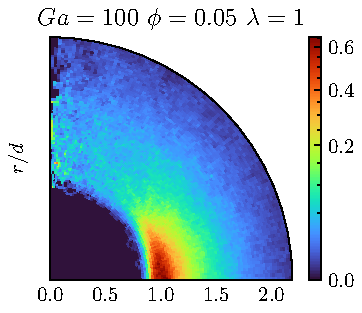
\includegraphics[height=0.3\textwidth]{image/HOMOGENEOUS_NEW/Dist/Pnst_l_1_Ga_100_PHI_0_05.pdf}};
    \draw[red,very thick] (img.south west) rectangle (img.north east);
    \draw[very thick,->] (img2) --(img);
    % \node (2D) at (img.south){$P_\text{nst}(r,\theta)$};
    \node[below= 0.5cm of img] {2D pdf in polar coordinate $P_\text{nst}(r,\theta)$};
  \end{tikzpicture}

\end{frame}

\begin{frame}
  \frametitle{Nearest pair Probability Density Function}

  \begin{columns}
    \column{0.7\textwidth}
    \centering
    \begin{tabular}{cccc}
      &
      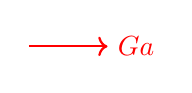
\begin{tikzpicture}[color=red]
        \draw[thick,->] (0,0) -- (1,0)node[right]{$Ga$};
      \end{tikzpicture}& & \\ 
        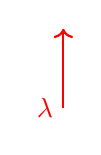
\begin{tikzpicture}[color=red]
          \draw[thick,<-] (0,0) -- (0,-1)node[left]{$\lambda$};
        \end{tikzpicture} 
        &
        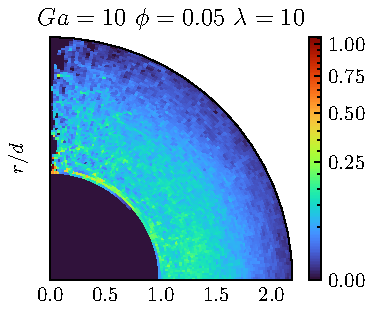
\includegraphics[height=0.3\textwidth]{image/HOMOGENEOUS_NEW/Dist/Pnst_l_10_Ga_10_PHI_0_05.pdf}  &
        % 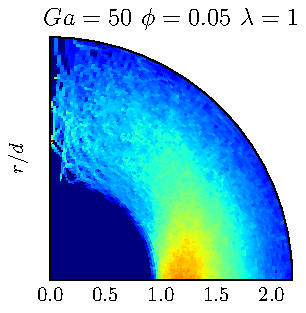
\includegraphics[height=0.3\textwidth]{image/HOMOGENEOUS_NEW/Dist/Pnst_l_1_Ga_50_PHI_0_05.pdf} &
        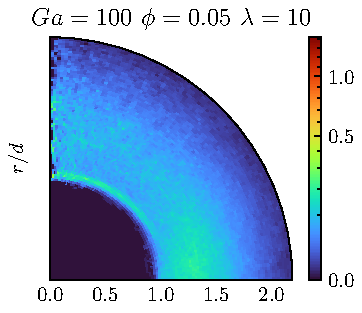
\includegraphics[height=0.3\textwidth]{image/HOMOGENEOUS_NEW/Dist/Pnst_l_10_Ga_100_PHI_0_05.pdf} 
        \\
         &
          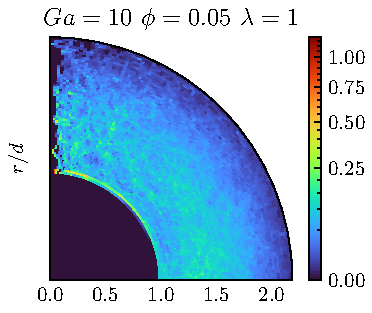
\includegraphics[height=0.3\textwidth]{image/HOMOGENEOUS_NEW/Dist/Pnst_l_1_Ga_10_PHI_0_05.pdf} &
        % 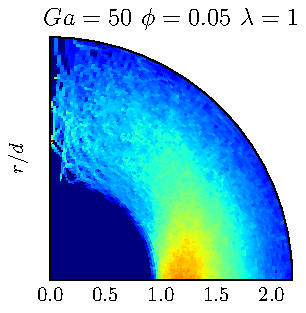
\includegraphics[height=0.3\textwidth]{image/HOMOGENEOUS_NEW/Dist/Pnst_l_1_Ga_50_PHI_0_05.pdf}&
        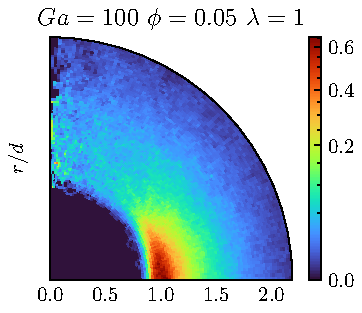
\includegraphics[height=0.3\textwidth]{image/HOMOGENEOUS_NEW/Dist/Pnst_l_1_Ga_100_PHI_0_05.pdf}\\
      \end{tabular}

      \column{0.3\textwidth}
      \begin{figure}
        \caption{Plots of $P_{nst} (\textbf{r})$ for different $Ga$ and $\phi$.}
      \end{figure}
    
    \begin{itemize}
      \item Drafting-Kissing-Tumbling mechanism for low $\lambda$ and high $Ga$. 
    \end{itemize}
  \end{columns}
  $\to$ The viscosity ratio $\lambda$ greatly influences the microstructure
\end{frame}

\begin{frame}
  \frametitle{Consequence on the particule arrangements}

  \begin{figure}[h!]
    \centering
    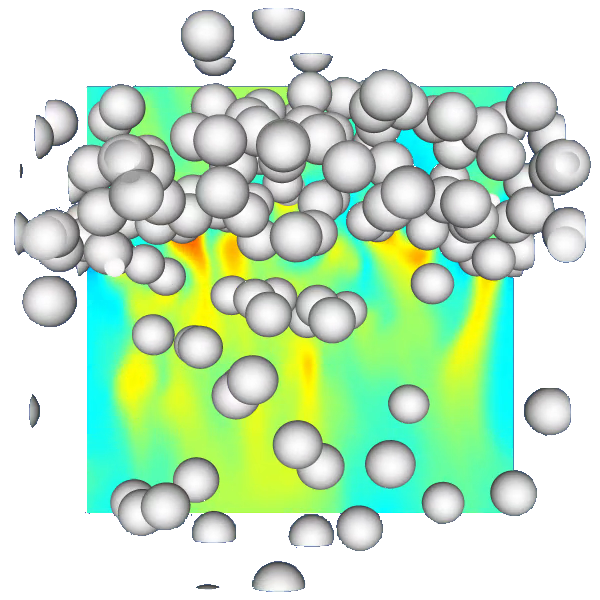
\includegraphics[width=0.45\textwidth]{image/HOMOGENEOUS_NEW/P_PHI_5_l_10_Ga_100.png}
    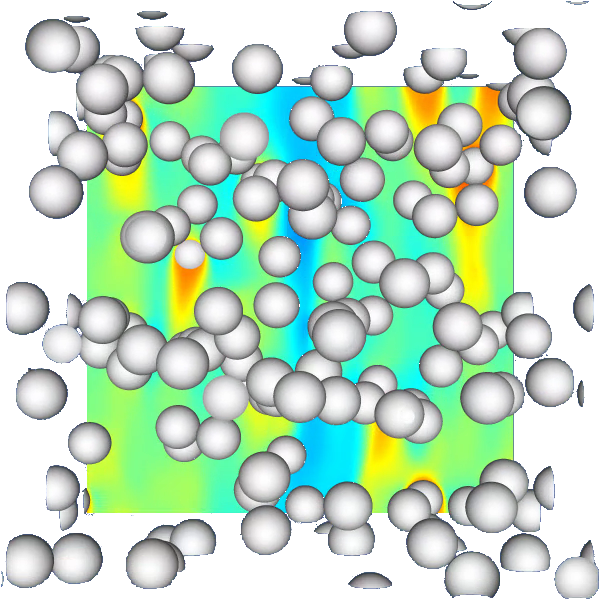
\includegraphics[width=0.45\textwidth]{image/HOMOGENEOUS_NEW/P_PHI_5_l_1_Ga_100.png}
 %    \includegraphics[width=0.45\textwidth]{image/HOMOGENEOUS_NEW/Ga_100_phi_005_l_10.png}
    \caption{Snapshot of a simulation at $t^* = 150$ for $\phi=0.05$ and $Ga=100$.
      Color map: values of the vertical component of the velocity field on the vertical plane at $z=0$.
      \break
    (left)  $\lambda = 1$.
    (right)  $\lambda = 10$.
    }
    \label{fig:images}
 \end{figure}

\end{frame}


\begin{frame}
  {A concise way to describe the microstructure}
\footnotesize
  We use the second moment of the pair distribution: 
  \begin{align*}
    \textbf{R} = \int \textbf{rr} P_{nst}(\textbf{r}) d\textbf{r}
    &&
    \textbf{A} = 
    \textbf{R} - \frac{1}{3}(\textbf{R}: \textbf{I}) \textbf{I}
  \end{align*}
\begin{figure}
  \centering
  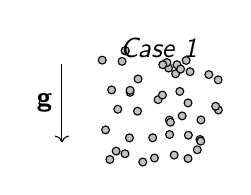
\begin{tikzpicture}[scale=0.5]
  \draw[->] (-1,2.5)--++(0,-2)node[midway, left]{$\textbf{g}$};
  \foreach \i in {1,...,5} {
  \pgfmathsetmacro{\x}{rnd}
  \pgfmathsetmacro{\y}{rnd}
  \draw[fill=gray!50] ($(\x,\y)$) circle (0.1);
  }
  \foreach \i in {1,...,5} {
  \pgfmathsetmacro{\x}{rnd}
  \pgfmathsetmacro{\y}{rnd}
  \draw[fill=gray!50] ($(\x+1,\y)$) circle (0.1);
  }
  \foreach \i in {1,...,5} {
  \pgfmathsetmacro{\x}{rnd}
  \pgfmathsetmacro{\y}{rnd}
  \draw[fill=gray!50] ($(\x+2,\y)$) circle (0.1);
  }
  \foreach \i in {1,...,5} {
      \pgfmathsetmacro{\x}{rnd}
      \pgfmathsetmacro{\y}{rnd}
      \draw[fill=gray!50] ($(\x+1,\y+1)$) circle (0.1);
  }
  \foreach \i in {1,...,5} {
  \pgfmathsetmacro{\x}{rnd}
  \pgfmathsetmacro{\y}{rnd}
  \draw[fill=gray!50] ($(\x+2,\y+1)$) circle (0.1);
  }
  \foreach \i in {1,...,5} {
  \pgfmathsetmacro{\x}{rnd}
  \pgfmathsetmacro{\y}{rnd}
  \draw[fill=gray!50] ($(\x,\y+1)$) circle (0.1);
  }
  \foreach \i in {1,...,5} {
      \pgfmathsetmacro{\x}{rnd}
      \pgfmathsetmacro{\y}{rnd}
      \draw[fill=gray!50] ($(\x+1,\y+2)$) circle (0.1);
  }
  \foreach \i in {1,...,5} {
  \pgfmathsetmacro{\x}{rnd}
  \pgfmathsetmacro{\y}{rnd}
  \draw[fill=gray!50] ($(\x+2,\y+2)$) circle (0.1);
  }
  \foreach \i in {1,...,5} {
  \pgfmathsetmacro{\x}{rnd}
  \pgfmathsetmacro{\y}{rnd}
  \draw[fill=gray!50] ($(\x,\y+2)$) circle (0.1);
  }
  \draw (1.5,3.4)node[below]{\textit{Case 1}};
\end{tikzpicture}
\hfill
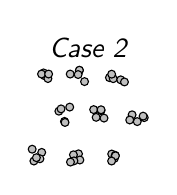
\begin{tikzpicture}[scale=0.5]
  \foreach \i in {1,...,5} {
  \pgfmathsetmacro{\x}{rnd*0.4}
  \pgfmathsetmacro{\y}{rnd*0.4}
  \draw[fill=gray!50] ($(\x,\y)$) circle (0.1);
  }
  \foreach \i in {1,...,5} {
  \pgfmathsetmacro{\x}{rnd*0.3}
  \pgfmathsetmacro{\y}{rnd*0.3}
  \draw[fill=gray!50] ($(\x+1,\y)$) circle (0.1);
  }
  \foreach \i in {1,...,5} {
  \pgfmathsetmacro{\x}{rnd*0.3}
  \pgfmathsetmacro{\y}{rnd*0.3}
  \draw[fill=gray!50] ($(\x+2,\y)$) circle (0.1);
  }
  \foreach \i in {1,...,5} {
      \pgfmathsetmacro{\x}{rnd*0.5}
      \pgfmathsetmacro{\y}{rnd*0.5}
      \draw[fill=gray!50] ($(\x+0.5,\y+1)$) circle (0.1);
  }
  \foreach \i in {1,...,5} {
      \pgfmathsetmacro{\x}{rnd*0.4}
      \pgfmathsetmacro{\y}{rnd*0.4}
      \draw[fill=gray!50] ($(\x+2.5,\y+1)$) circle (0.1);
  }
  \foreach \i in {1,...,5} {
      \pgfmathsetmacro{\x}{rnd*0.4}
      \pgfmathsetmacro{\y}{rnd*0.4}
      \draw[fill=gray!50] ($(\x+1.5,\y+1)$) circle (0.1);
      }
  \foreach \i in {1,...,5} {
      \pgfmathsetmacro{\x}{rnd*0.5}
      \pgfmathsetmacro{\y}{rnd*0.5}
      \draw[fill=gray!50] ($(\x,\y+2)$) circle (0.1);
  }
  \foreach \i in {1,...,5} {
      \pgfmathsetmacro{\x}{rnd*0.4}
      \pgfmathsetmacro{\y}{rnd*0.4}
      \draw[fill=gray!50] ($(\x+2,\y+2)$) circle (0.1);
  }
  \foreach \i in {1,...,5} {
      \pgfmathsetmacro{\x}{rnd*0.4}
      \pgfmathsetmacro{\y}{rnd*0.4}
      \draw[fill=gray!50] ($(\x+1,\y+2)$) circle (0.1);
      }
  \draw (1.5,3.4)node[below]{\textit{Case 2}};
\end{tikzpicture}
\hfill
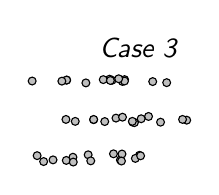
\begin{tikzpicture}[scale=0.5]
  \foreach \i in {1,...,5} {
  \pgfmathsetmacro{\x}{rnd*1.5}
  \pgfmathsetmacro{\y}{rnd*0.2}
  \draw[fill=gray!50] ($(\x,\y)$) circle (0.1);
  }
  \foreach \i in {1,...,5} {
  \pgfmathsetmacro{\x}{rnd*1.5}
  \pgfmathsetmacro{\y}{rnd*0.3}
  \draw[fill=gray!50] ($(\x+1,\y)$) circle (0.1);
  }
  \foreach \i in {1,...,5} {
  \pgfmathsetmacro{\x}{rnd*1.5}
  \pgfmathsetmacro{\y}{rnd*0.3}
  \draw[fill=gray!50] ($(\x+2,\y)$) circle (0.1);
  }
  \foreach \i in {1,...,5} {
      \pgfmathsetmacro{\x}{rnd*1.5}
      \pgfmathsetmacro{\y}{rnd*0.2}
      \draw[fill=gray!50] ($(\x+1+0.5,\y+1)$) circle (0.1);
  }
  \foreach \i in {1,...,5} {
  \pgfmathsetmacro{\x}{rnd*1.5}
  \pgfmathsetmacro{\y}{rnd*0.2}
  \draw[fill=gray!50] ($(\x+2+0.5,\y+1)$) circle (0.1);
  }
  \foreach \i in {1,...,5} {
  \pgfmathsetmacro{\x}{rnd*1.5}
  \pgfmathsetmacro{\y}{rnd*0.1}
  \draw[fill=gray!50] ($(\x+0.5,\y+1)$) circle (0.1);
  }
  \foreach \i in {1,...,5} {
      \pgfmathsetmacro{\x}{rnd*1.5}
      \pgfmathsetmacro{\y}{rnd*0.2}
      \draw[fill=gray!50] ($(\x+1,\y+2)$) circle (0.1);
  }
  \foreach \i in {1,...,5} {
  \pgfmathsetmacro{\x}{rnd*1.5}
  \pgfmathsetmacro{\y}{rnd*0.2}
  \draw[fill=gray!50] ($(\x+2,\y+2)$) circle (0.1);
  }
  \foreach \i in {1,...,5} {
  \pgfmathsetmacro{\x}{rnd*1.5}
  \pgfmathsetmacro{\y}{rnd*0.1}
  \draw[fill=gray!50] ($(\x,\y+2)$) circle (0.1);
  }
  \draw (1.5,3.4)node[below right]{\textit{Case 3}};
\end{tikzpicture}
\end{figure}
\begin{table}[h!]
  \caption{Microstructure classification}
  \label{tab:microstructure}
  \centering
  \begin{tabular}{|lccccc|} \hline
      Microstructure types & Homogeneous & Isotropic & Figure & $\textbf{R}:\textbf{I}/r_m^2$ & $A_{xx}/tr(\textbf{R})$ \\
      Homogeneous & Yes & Yes &(\textit{Case 1}) & $ \approx 1$ & $\approx 0$ \\
      Dispersed &  No & Yes  &(\textit{Case 2}) & $ > 1$ & $\approx 0$ \\
      Clustering &  No & Yes  &(\textit{Case 2}) & $ < 1$ & $\approx 0$ \\
      Layering &    No & No  &(\textit{Case 3}) & $ - $ & $< 1$\\ \hline
  \end{tabular}
\end{table}

\end{frame}


\begin{frame}
  \frametitle{Phase diagram of the microstructure anisotropy}
  \footnotesize
  % \begin{align*}
  %   \textbf{R} = \int \textbf{rr} P_{nst}(\textbf{r}) d\textbf{r}
  %   &&
  %   \textbf{A} = 
  %   \textbf{R} - \frac{1}{3}(\textbf{R}: \textbf{I}) \textbf{I}
  % \end{align*}
  \begin{figure}[h!]
    \centering
    % \begin{tikzpicture}[scale=0.5]
    %     \node (img) at (0,0) {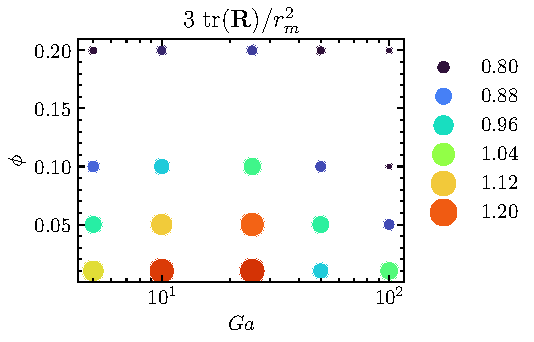
\includegraphics[height=0.3\textwidth]{image/HOMOGENEOUS_NEW/PA/phase_Rtr_l_1.pdf}};
    %     % \draw[dashed] (10cm,-1.6) ellipse (3 and 2);
    %     \node (txt) at (-2,1) {Clustering};
    %     \node (txt) at (-1,-1.6) {Dispersed};
    %     \draw[dashed] ($(-1,-1.6) + (-10:3 and 2)$(P) arc
    %     (-10:155:3 and 2);
    %     \node (img) at (10.5,0) {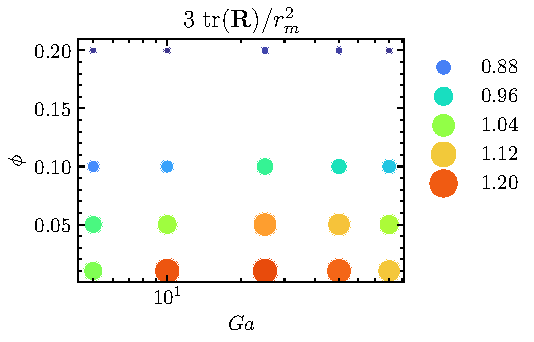
\includegraphics[height=0.3\textwidth]{image/HOMOGENEOUS_NEW/PA/phase_Rtr_l_10.pdf}};
    %     % \draw[dashed] (10cm,-1.6) ellipse (3 and 2);
    %     \node (txt) at (8.5,1) {Clustering};
    %     \node (txt) at (10,-1.6) {Dispersed};
    %     \draw[dashed] ($(10,-2) + (-10:3 and 2)$(P) arc
    %     (-10:180:3 and 2);
    % \end{tikzpicture}
    \begin{tikzpicture}[scale=0.5]
        \node (img) at (0,0) {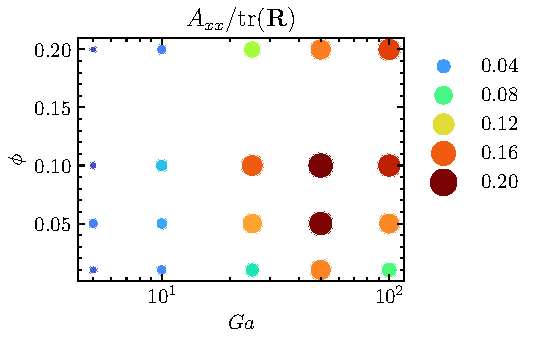
\includegraphics[height=0.3\textwidth]{image/HOMOGENEOUS_NEW/PA/phase_axx_l_1.pdf}};
        \draw[dashed] (1.4,0.3) ellipse (1.5 and 2.5);
        \node (txt) at (1.4,1) {Anisotropic};
        \node (txt) at (-2,1) {Isotropic};

        \node (img) at (10.5,0) {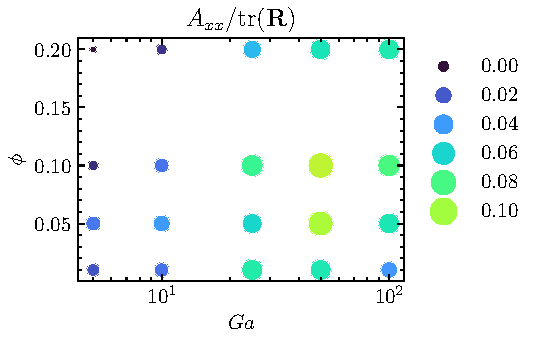
\includegraphics[height=0.3\textwidth]{image/HOMOGENEOUS_NEW/PA/phase_axx_l_10.pdf}};
        % \draw[dashed] (11.7,-0.5) ellipse (0.75 and 1.75);
        % \node (txt) at (11.7,1) {Anisotropic};
        \node (txt) at (8,1) {Isotropic};
    \end{tikzpicture}
    \caption{
        % (top) Phase diagram of the dimensionless mean square distance to the nearest neighbor, $\textbf{I}:\textbf{R}/r_m^2$.
         Phase diagram of the dimensionless horizontal components of the anisotropy tensor, $A_{xx}/\text{tr}(\textbf{R})$.  
        (left) Iso-viscosity emulsion $\lambda = 1$.
        (right) Viscous droplets $\lambda = 10$. }
    \label{fig:phase}
\end{figure}

$\to$ Iso-viscosity emulsions exhibit anisotropic clusters at $Ga > 25$ and $\phi \ge 0.05$.  

\end{frame}

\begin{frame}
  {A transport equation to describe the evolution of the microstructure}
  We could show that $\textbf{R}$ obeys the transport equation: 
\begin{equation*}
    \pddt (n_p\textbf{R})
    + \div [
      n_p(\textbf{u}_p\textbf{R}
    + \textbf{R}^\text{Re})]
    = 
    - \frac{n_p\textbf{R}}{a_p}
    +n_p\textbf{B}
    + n_p\textbf{D}
    + n_p\textbf{W}
\end{equation*}
With the ``relative velocity production term''
\begin{align*}
    % n_p \textbf{R}^\text{Re}(\textbf{x},t)
    % =
    % \int_{0}^\infty
    % \int_{\mathbb{R}^3}
    % \textbf{rr}(\textbf{u}^\text{nst}_p - \textbf{u}_p)
    % P(\textbf{x},\textbf{r},t,a)
    % d\textbf{r}da,\\
    % n_p \textbf{B}(\textbf{x},t)
    % =
    % \int_{0}^\infty
    % \int_{\mathbb{R}^3}
    % \textbf{rr}
    % P(\textbf{x},\textbf{r},t,0)\delta(a)
    % d\textbf{r}da, \\
    % n_p\textbf{D}(\textbf{x},t) = 
    % \int_{0}^\infty
    % \int_{\mathbb{R}^3} \textbf{rr}
    % \left[
    %     \frac{1}{a_p(\textbf{x},t)}
    %     - \frac{1}{\tau^\text{nst}(\textbf{x},\textbf{r},t,a)}
    % \right]
    % P_\text{nst}
    % d\textbf{r}
    % da,\\
    n_p \textbf{W}(\textbf{x},t) = 
    \int_{0}^\infty
    \int_{\mathbb{R}^3} \left[
        \textbf{r} \textbf{w}^\text{nst}_p
        + \textbf{w}^\text{nst}_p\textbf{r}
    \right]P_\text{nst}
    d\textbf{r}
    da.
\end{align*} 

\begin{itemize}
  \item  $\textbf{w}^\text{nst}_p(\textbf{x},\textbf{r},t,a)$ is the averaged relative velocity between two nearest neighboring particules, one of which is situated at $\textbf{x}$ and time $t$, with its nearest neighbor at $\textbf{x}+\textbf{r}$ with age $a$. 
  \item \textbf{R} relaxes on a timescale $a_p$ which is related to the particule interaction time.
\end{itemize}

$\to$ The relative approach velocity $\textbf{w}^\text{nst}_p$, and the mean age of interaction $a_p$ seems primordial in the evolution of \textbf{R}. 

\end{frame}


\begin{frame}{Mean time of interaction between droplets}
  \begin{figure}[h!]
    \centering
    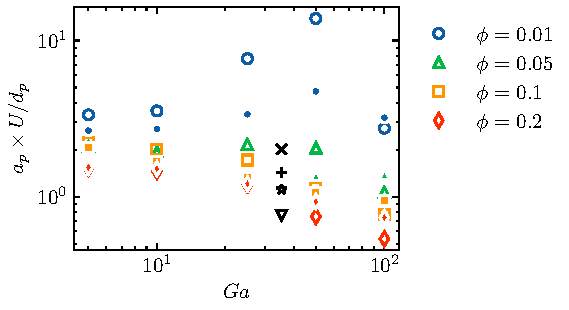
\includegraphics[height = 0.3\textwidth]{image/HOMOGENEOUS_NEW/PA/age.pdf}
    % 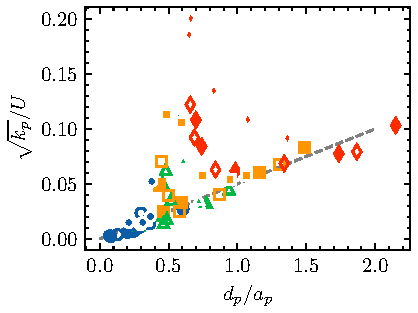
\includegraphics[height = 0.3\textwidth]{image/HOMOGENEOUS_NEW/PA/Corr.pdf}
    % 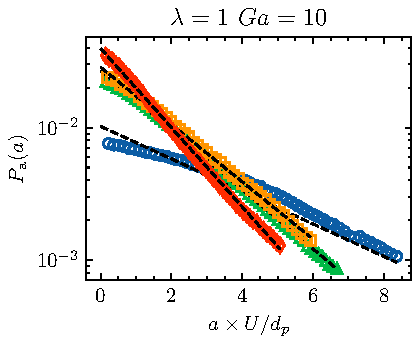
\includegraphics[height = 0.3\textwidth]{image/HOMOGENEOUS_NEW/Dist/Pa_l_1_Ga_10.pdf}
    % 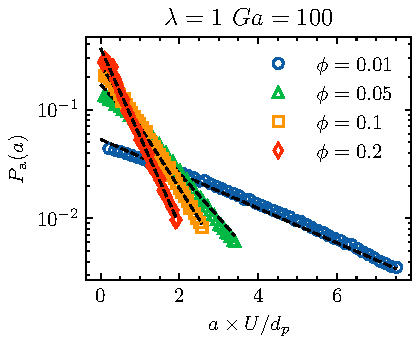
\includegraphics[height = 0.3\textwidth]{image/HOMOGENEOUS_NEW/Dist/Pa_l_1_Ga_100.pdf}
    \caption{
    (left) Mean dimensionless age $a_p =  \int_0^\infty aP_a(\textbf{x},t,a)da$ in terms of the \textit{Galileo} number for different volume fraction :   
    ($\pmb\bigcirc$) $\phi = 0.01$; ($\pmb\triangle$) $ \phi = 0.05$; ($\pmb\square$) $\phi = 0.1$ ($\pmb\lozenge$) $\phi = 0.2$.
    The hollow symbols correspond to $\lambda = 1$, the filled symbols to $\lambda = 10$.
    Black symbols represent the DNS results of (Zhang et al. (2023)) for hard sphere suspension with $\phi = 0.0168,0.0565,0.1341,0.2622$, corresponding to the symbols : $\pmb\times, \pmb +, \pmb\star , \pmb\triangledown$, respectively.
    }
    \label{fig:tau_p}
\end{figure}
\end{frame}

\begin{frame}{Relative normal approach velocity}

\only<1>
{
  \begin{figure}[h!]
    \centering
    \begin{tikzpicture}[ scale = 0.6]
        \node (img) at (-0.7\textwidth,0){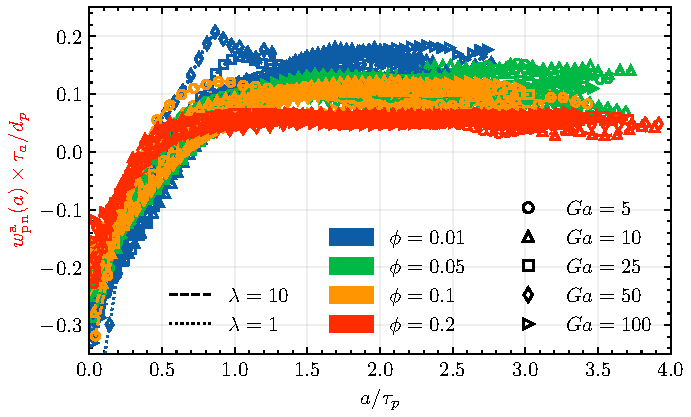
\includegraphics[height = 0.35\textwidth]{image/HOMOGENEOUS_NEW/Age_cond/uR_rel2.pdf}};
        \filldraw[ gray!50!white](0,0) circle (0.5);
        \filldraw[ gray!50!white](1,3)circle (0.5);
        \draw(0,0)node[right]{$\textbf{x}_i$};
        \draw[dashed](0,0)--(1,3)node[right]{$\textbf{x}_j$};
        % \draw[very thick,<-,blue](-1,0)--++(0,1)node[right]{$\bm{b}$};
        \draw[very thick,->](1,3)--++(0.9,-1.8)node[above right]{$\textbf{w}^\text{nst}(a)$};
        \draw[very thick,->,red](1,3)--++(-0.5,-1.5)node[left]{$w_{ij,n}(a)$};
        \draw[dashed](1,3)++(0.9,-1.8) -- (1,3)++(-0.5,-1.5);
        \node (ii) at (1,-1){$\textbf{w}_{ij} = \textbf{u}_j - \textbf{u}_i$};
        \node (ii) at (1,-1.6){$w_{ij,n} = \textbf{w}_{ij}\cdot \textbf{r}/|\textbf{r}|$};
    \end{tikzpicture} 
\end{figure}
  The theoretical observations suggest that in a statistically steady-state regime :
\begin{equation}
  \int_\mathbb{R} w_{pn}^aP_a(\textbf{x},t,a) da = 0 
\end{equation}
}
\only<2>
{   
  \begin{figure}[h!]
    \centering
    \begin{tikzpicture}[ scale = 0.6]
      % \only<1>\node (img) at (-0.7\textwidth,0){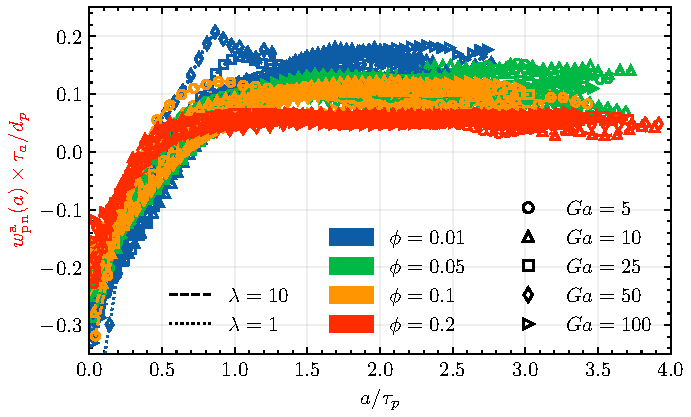
\includegraphics[height = 0.35\textwidth]{image/HOMOGENEOUS_NEW/Age_cond/uR_rel2.pdf}};
      \node (img) at (-0.7\textwidth,0){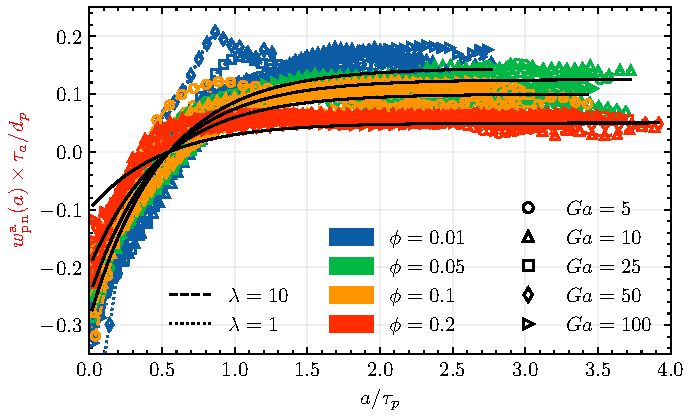
\includegraphics[height = 0.35\textwidth]{image/HOMOGENEOUS_NEW/Age_cond/uR_rel.pdf}};
      \filldraw[ gray!50!white](0,0) circle (0.5);
      \filldraw[ gray!50!white](1,3)circle (0.5);
      \draw(0,0)node[right]{$\textbf{x}_i$};
      \draw[dashed](0,0)--(1,3)node[right]{$\textbf{x}_j$};
      % \draw[very thick,<-,blue](-1,0)--++(0,1)node[right]{$\bm{b}$};
      \draw[very thick,->](1,3)--++(0.9,-1.8)node[above right]{$\textbf{w}^\text{nst}(a)$};
      \draw[very thick,->,red](1,3)--++(-0.5,-1.5)node[left]{$w_{ij,n}(a)$};
      \draw[dashed](1,3)++(0.9,-1.8) -- (1,3)++(-0.5,-1.5);
      \node (ii) at (1,-1){$\textbf{w}_{ij} = \textbf{u}_j - \textbf{u}_i$};
      \node (ii) at (1,-1.6){$w_{ij,n} = \textbf{w}_{ij}\cdot \textbf{r}/|\textbf{r}|$};
    \end{tikzpicture} 
\end{figure}
  \begin{equation}
  w_{pn}^a(\textbf{x},t,a) = \frac{d_p}{\tau_p} 
  \left(
      0.15
      -\frac{\phi}{2}
  \right)\left(
      1 - 3e^{-2a/\tau_p}
  \right).
\end{equation}
}
\end{frame}



\section{Conclusion}
\section*{}



\end{document}
